%%%%%%%%%%%%%%%%%%%% author.tex %%%%%%%%%%%%%%%%%%%%%%%%%%%%%%%%%%%
%
% sample root file for your "contribution" to a proceedings volume
%
% Use this file as a template for your own input.
%
%%%%%%%%%%%%%%%% Springer %%%%%%%%%%%%%%%%%%%%%%%%%%%%%%%%%%


\documentclass{svproc}
%
% RECOMMENDED %%%%%%%%%%%%%%%%%%%%%%%%%%%%%%%%%%%%%%%%%%%%%%%%%%%
%

% to typeset URLs, URIs, and DOIs
\usepackage{url}
\def\UrlFont{\rmfamily}
\usepackage{amsmath}
\usepackage{graphicx}
\usepackage{mathtools}
\usepackage{gensymb}
% \usepackage{caption}
% \usepackage{subcaption}

\newtheorem{observation}{Observation}

\newenvironment{sketch}{%
  \renewcommand{\proofname}{Proof Sketch}\proof}{\endproof}

\DeclareMathOperator{\atantwo}{atan2}
\DeclareMathOperator{\sign}{sign}
\DeclareMathOperator{\sense}{sense}
\DeclarePairedDelimiter{\norm}{\lVert}{\rVert}

\begin{document}
\mainmatter              % start of a contribution
%
\title{Calculating the Segmented Helix Formed by Repetitions of Identical Subunits}
%
\titlerunning{Hamiltonian Mechanics}  % abbreviated title (for running head)
%                                     also used for the TOC unless
%                                     \toctitle is used
%
\titlerunning{Calculating the Segmented Helix}

\institute{Public Invention, Austin, TX 78704, USA,\\
\email{read.robert@gmail.com},\\ WWW home page:
\texttt{https://www.pubinv.org}
}

\author{Robert L. Read\inst{1}}

%% \author{Ivar Ekeland\inst{1} \and Roger Temam\inst{2}
%% Jeffrey Dean \and David Grove \and Craig Chambers \and Kim~B.~Bruce \and
%% Elsa Bertino}
%
\authorrunning{Robert L. Read}
%% \authorrunning{Ivar Ekeland et al.} % abbreviated author list (for running head)
%
%%%% List of authors for the TOC (use if author list has to be modified)
\tocauthor{Robert L. Read}
%
%% \institute{Princeton University, Princeton NJ 08544, USA,\\
%% \email{I.Ekeland@princeton.edu},\\ WWW home page:
%% \texttt{http://users/\homedir iekeland/web/welcome.html}
%% \and
%% Universit\'{e} de Paris-Sud,
%% Laboratoire d'Analyse Num\'{e}rique, B\^{a}timent 425,\\
%% F-91405 Orsay Cedex, France}

\maketitle              % typeset the title of the contribution

\begin{abstract}

  Eric Lord has observed:
\begin{quote}
  In nature, helical structures arise when identical structural subunits combine sequentially, the orientational and translational relation between each unit
  and its predecessor remaining constant.\citation{lord2002helical}
\end{quote}
A complete version of this paper proves this\citation{readfullsegmentedhelix}.
If a robot is composed of modular structural subunits that can change their shape or relation, the shape of the robot
can change. If they all change in the same way, the robot will be a segmented helix of varying length and curvature.
Closed-form expressions are given for the parameters of
the segmented helix generated from the intrinsic properties of a chained object and its
conjoining rule.
The construction of these from the rule for conjoining repeated subunits of arbitrary shape is provided,
allowing the complete parameters describing the unique
segmented helix generated by arbitrary stackings to be easily calculated.
Free-libre open-source interactive software and a website is provided which performs this computation
for arbitrary prisms along with interactive 3D visualization\cite{segmentedhelixinteractive}.
A theorem, proved in a longer version\cite{readfullsegmentedhelix}, is stated that any chain
can be transformed continuously between a toroid-like helix and a maximally-extended helix
by varying joint-face normal twist.
% We would like to encourage you to list your keywords within
% the abstract section using the \keywords{...} command.
\keywords{solid geometry, segmented helix, robotics, chemistry}
\end{abstract}
%

\section{Introduction}

The participants of the Public Invention Mathathon of 2018\cite{read2019mathathon} noticed:
\begin{observation}[Lord's Observation]
  “In nature, helical structures arise when identical structural subunits combine sequentially, the orientational and translational relation between each unit and its predecessor remaining constant.”\cite{lord2002helical}
  \label{obs:lords}
\end{observation}
Having found no earlier articulation of this statement
in writing, it is justified to name it after its earliest known author.
The purpose of this paper is to provide mathematical
tools and software for studying arbitrary
structures generated in this way, which are modeled as segmented helices.
A proof of Lord's Observation is provided in a longer version\cite{readfullsegmentedhelix}.
An interactive, 3D rendering website written in JavaScript which allows both calculation and
interactive play and study is provided\cite{segmentedhelixinteractive}
(see Figure \ref{fig:prismatic}).

\begin{figure}
  \centering
  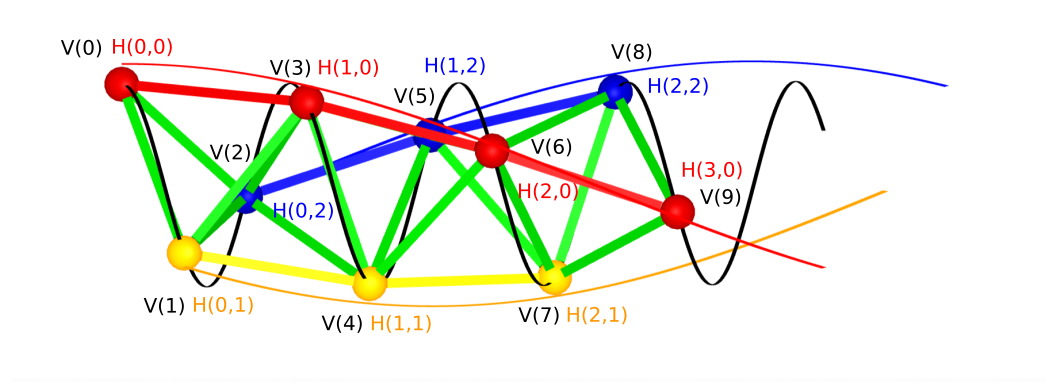
\includegraphics[width=0.7\textwidth]{figures/UnifiedDrawing.png}
  \caption{Tetrahelix\label{fig:helixnodes}}
  \includegraphics[width=0.7\textwidth]{figures/MedCantedCropped.png}
  \caption{The 7-tet Public Invention Tetrobot\label{fig:tetrobot}}
\end{figure}

Lord's Observation is exploited to discover symmetry which allows us to compute the helix when subunits are joined face-to-face with
the same {\em twist.}
This concept can be generalized to a {\em joint face angle}, even if the
objects conjoined do not technically have flat faces.
Varying the {\em twist} of the joint faces through a complete rotation produces a smoothly varying
spectrum of shapes that always includes a torus-like shape and a
{\em zig-zag} planar segmented helix of maximal extent.
A robot thus constructed of identical modules which can change their shape, such as the Tetrobot of Figure \ref{fig:tetrobot}, allows the helix to coil and uncoil
predictably based on the math herein.

\begin{figure}
  \centering
  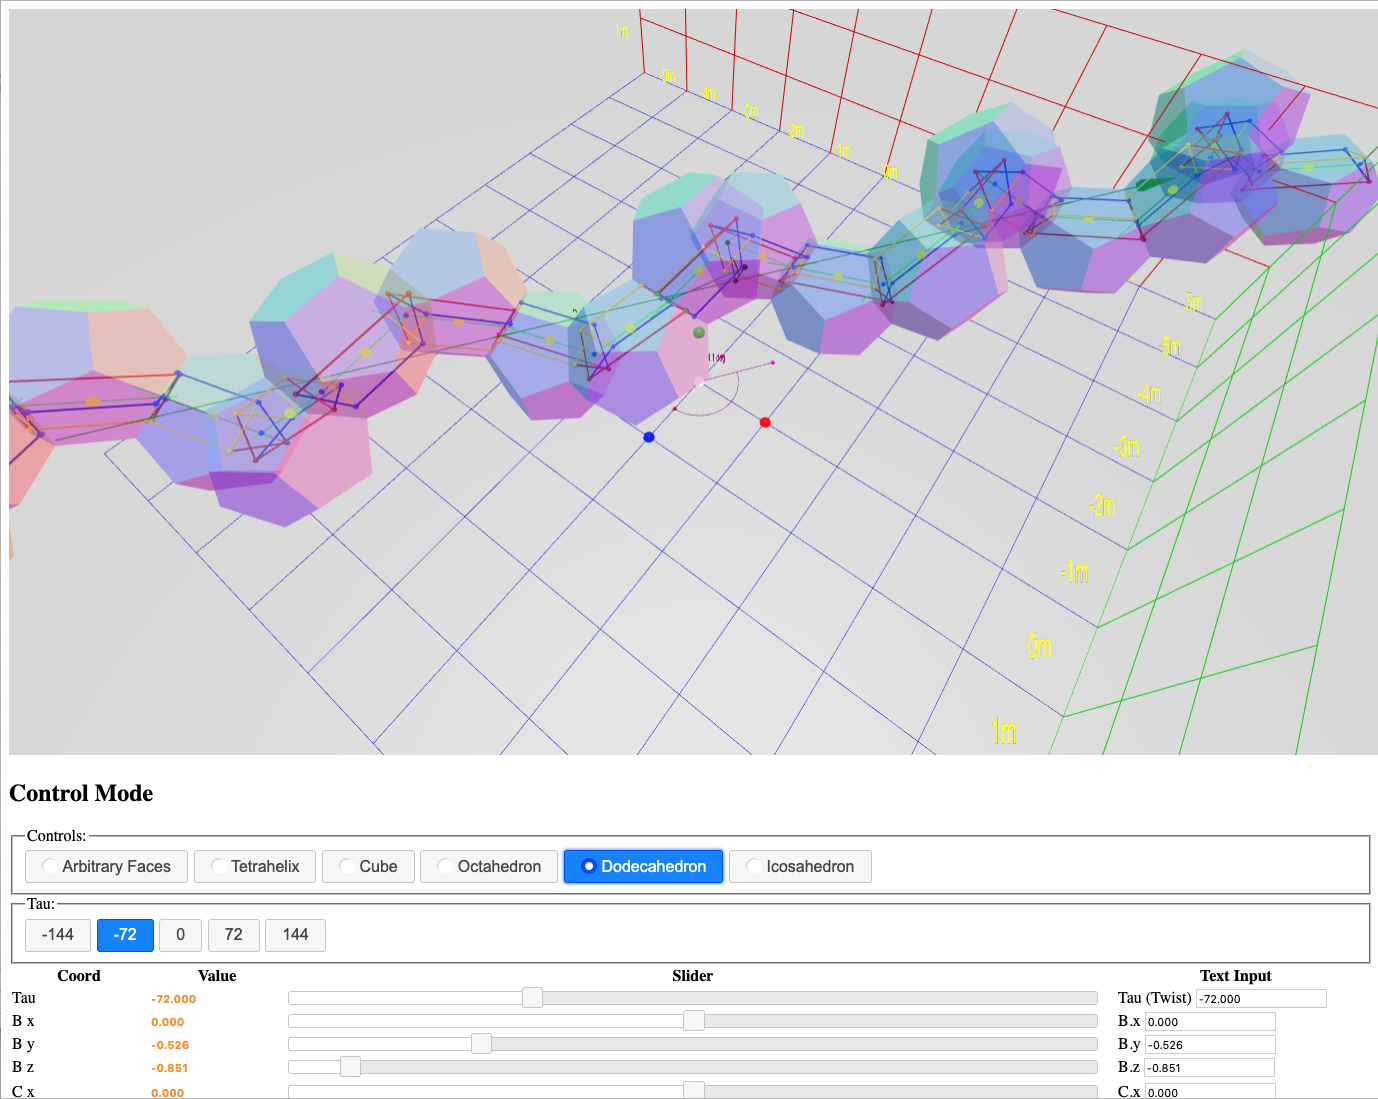
\includegraphics[width=0.5\textwidth]{figures/Dodecahedral.png}
 \caption{Screenshot: Segmented Helix Generated From the Dodecahedron}
  \label{fig:dodecahedron}
\end{figure}

\section{The Segmented Helix}

A chain of physical objects can be described by
calculating
the parameters for a continuous helix coincident on the joints by studying
a helix evaluated at integral points. Call such an object a {\em segmented helix}.
A segmented helix may be thought of as function that, given an integer, gives back a point in
3-space:
\begin{align}
    P_x(n) &= r \sin{n \theta}  \\
    P_y(n) &= r \cos{n \theta} \\
   P_z(n) &= n d
\end{align}

\begin{figure}
    \centering
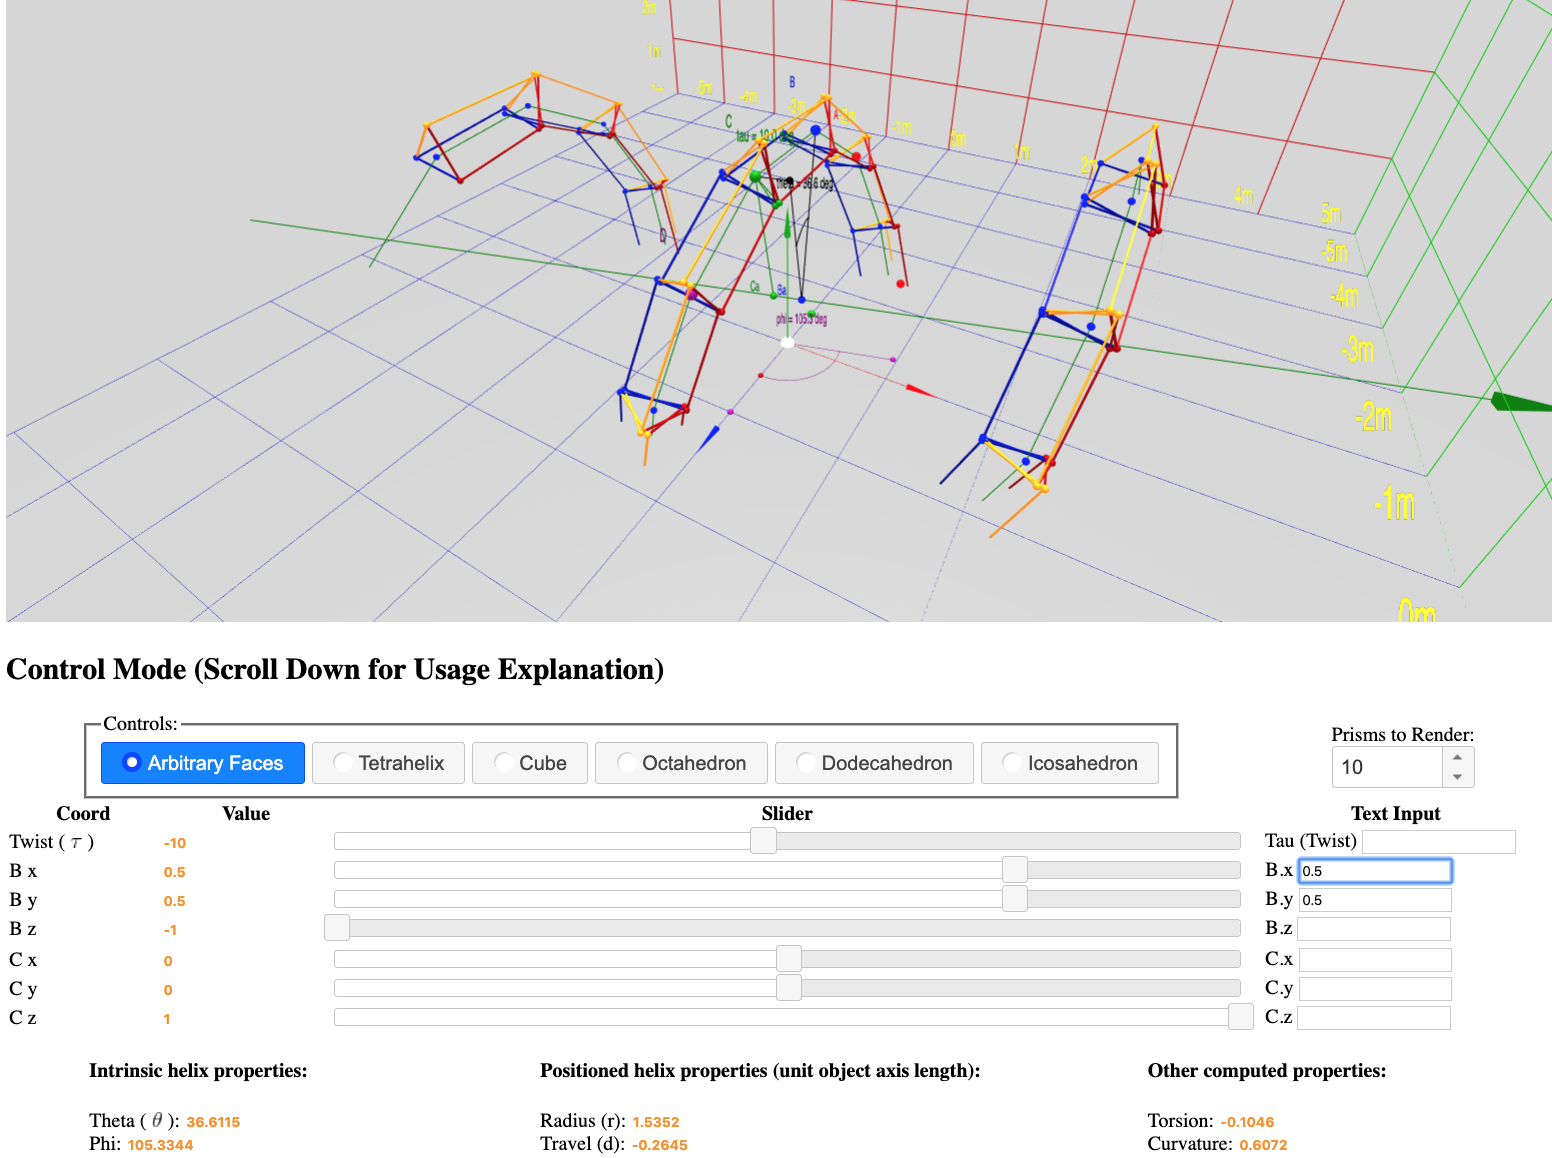
\includegraphics[width=0.6\textwidth]{figures/GeneralHelix.png}
\caption{Screenshot: A general (non-platonic) segmented helix from prisms\label{fig:prismatic}}
\end{figure}


There are two complementary ways of learning about such segmented helices.
In one approach (see {\em Point Axis} of Section \ref{sec:pointaxis})
we have knowledge of the segmented helix and
wish to learn about the subunits and the rule with which the subunits are combined.
In the other approach ({\em The Joint Face Normal Method} of Section \ref{sec:facenormal}),
one may know {\it a priori} exactly the
relevant properties of the objects and the rule with which they combine
and seek to compactly describe the segmented helix they create.

\begin{figure}
     \centering
          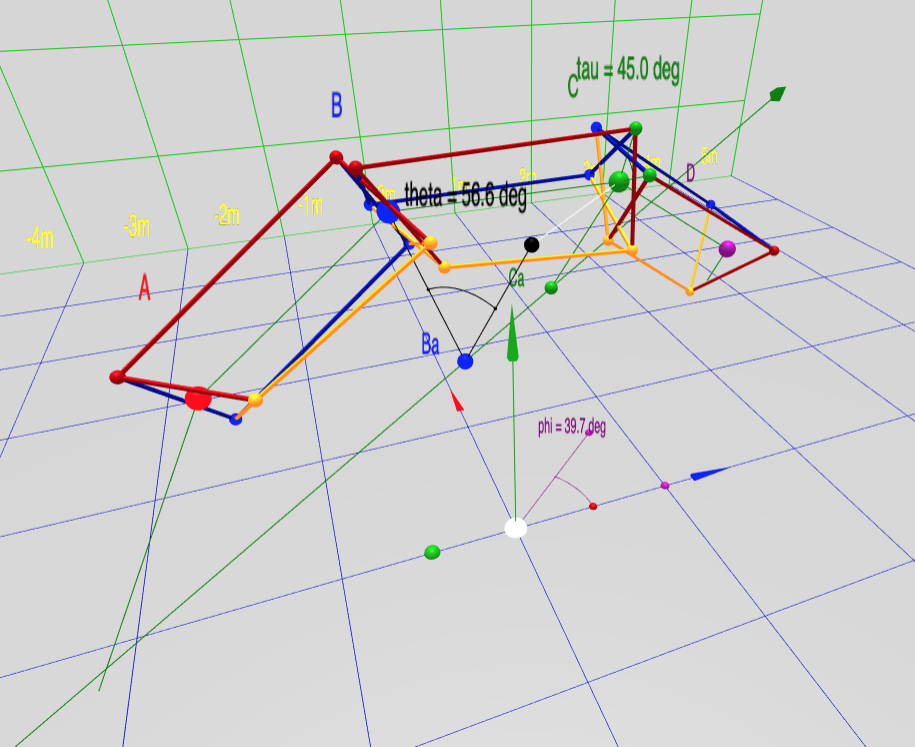
\includegraphics[width=0.6\textwidth]{figures/ABCDFigure.png}
     \caption{Naming of measures}
  \label{fig:naming}
\end{figure}

Figure \ref{fig:naming}, a screenshot, demonstrates naming convention and concepts.
An arbitrary repeated object is represented as a prism
with triangular cross-section,
thus representing face-to-face connection. Figure \ref{fig:prismatic} shows a long part of a segmented helix
built from prisms.

In this diagram, the
points $A,B,C$, and $D$ are represented by the sphere of the same color as the label. The view is roughly in the direction of
the axis of the segmented helix, which is drawn as a dark green arrow, pointing in the positive $z$ and positive $x$ direction,
parallel to the $XZ$-plane (Y is vertical).

In this canonical representation the object axis $\overrightarrow{BC}$ is
the $z$-axis.
$\theta$ is the rotation around the $z$-axis
between adjacent points, and
$r$ is the radius of the segmented helix.

Any point on the segmented helix has a closest point on the axis of the helix.
In particular, the points closest to the
joints $B$ and $C$ are called {\em joint axis points}, $B_a$ and $C_a$.
Then $d$ is the distance along the axis (travel) between consecutive joint axis points.

A segmented helix located in space is completely determined by
the three intrinsic parameters $r,d,\theta$, plus
a vector describing the axis
of the helix, and the position of any one joint.

The following concepts and conventional variable names for them will be related:
\begin{itemize}
\item $L$ is the distance between any two adjacent joints (between $B$ and $C$, for example).
  \item $c$ is the length of a chord formed by the projection of the segment between two points projected along the axis of the segmented helix (a chemist may recognize this as the distance between residues on a {\em helical wheel} projection).
\item $\phi$ is the angle between any vector between two adjacent joints and the axis of the helix. In physical screws used in mechanical engineering, this is analogous to the {\em helix angle}.
  \end{itemize}
Finally, we find it useful to define the {\em tightness t} of a segmented helix
as travel divided by radius, a number
analogous to the extension of a coil spring or slinky.
A torus-like segmented helix has zero tightness and a zig-zag has
maximum tightness.

These quantities are related:
\begin{align}
    c &= 2r\sin{\frac{\theta}{2}} \\
    L^2 &= c^2+d^2  \\
    \arctan{\frac{c}{d}}  &= \phi \\
    t &= d / r
\end{align}

\label{sec:SegmentedHelix}

\section{Periodic Chains Produce Segmented Helices}

Identical objects conjoined via a rule
produce {\em periodic chains} of objects that are uniformly intersected
by segmented helices.

Consider $N$ identical objects which each have two points, $A$ and $B$, called {\em joints}. Call
$\overrightarrow{AB}$ the {\em axis} of this object.
Consider the frame of reference for this object to have
its axis on the $z$-axis with $B$ in the positive direction, the
midpoint of the object being at the origin.

Consider any rule that conjoins $A$ of object $i+1$ to $B$ such that
from the frame of reference of $i$, the object $i+1$ and anything rigidly
attached to it is always in the same position in the frame of reference for $i$.
Informally, $i+1$ ``looks the same'' to $i$, no matter what $i$ is chosen, $i < N$.
Call a chain of $N$ identical rigid objects conjoined via a rule that
conjoins $A_{i+1}$ to $B_i$ in such a way that every vector
of $B$ is always in the same position relative to a frame of reference
constructed from $A$, a {\em periodic chain.}

\begin{theorem}[Segmented Helix]
  \label{thm:helix}
  Any periodic chain of three or more objects has a unique segmented helix
  whose segments
  lies on the axes of these objects.
\end{theorem}

A proof is provided in the longer version of this paper\cite{readfullsegmentedhelix}.
Because periodic chains are merely a clarification of ``identical structural subunits'',
this theorem proves Lord's Observation (Observation \ref{obs:lords}).

Note that Theorem \ref{thm:helix} is independent of the actual
shape or shapes of the objects joined, so long as the rule for joining them
is universal.

Because a helix may be degenerate, Theorem \ref{thm:helix} clarifies that
a periodic chain of objects may also be degenerate to the human eye, in that they may:
\begin{enumerate}
\item form a straight line,
\item be planar about a center, forming a polygon or ring, or
\item form a planar saw-tooth or zig-zag pattern of indefinite extent ($\theta = \pi$).
\end{enumerate}

\section{{\em PointAxis}: Computing Segmented Helices from Joints}
\label{sec:pointaxis}

Using tools from linear algebra \cite{kahn1989defining}, a sketch of finding the segmented helix from
four consecutive known points $A,B,C$, and $D$ ({\em PointAxis}), is:
\begin{itemize}
\item Construct a rigid transformation that places the points conveniently on the $z$-axis and balanced
  around the $y$-axis.
\item Compute the bisectors of the angle between object axes $ \angle{ABC}$, called $\overrightarrow{B_b}$ and the
  bisecting angle $\overrightarrow{C_b}$ of $\angle{BCD}$.
  If the points are collinear, they are a special case.
\item Because these angle bisectors point at the axis of the segmented helix, their cross product is a vector
  in the direction of the axis. If $\overrightarrow{B_b}$ and $\overrightarrow{C_b}$ are parallel or anti-parallel the cross product is not defined, requiring a modified calculation.
\item  Otherwise the vectors $\overrightarrow{B_b}$ and $\overrightarrow{C_b}$ are skew, and the algorithm for the closest points on
  two skew lines provides two axis points $B_a$ and $C_a$ on these vectors which
  are the closest points on those lines and are also points on the helix axis.
\item The distance between $B_a$ and $B$ is the radius, and the distance between $B_a$ and $C_a$ is the travel $d$ along the axis.
  \item The angle between $\overrightarrow{B - B_a}$ and $\overrightarrow{C - C_a}$ is $\theta$.
\end{itemize}

In order to use the {\em PointAxis} algorithm, we need a way
to compute points $A$ and $D$ in balance around the obect axis $\overrightarrow{BC}$. In the full paper\cite{readfullsegmentedhelix}
we state and sketch a proof of a lemma that the points $A$ and $D$ can always be brought into simplifying balance.

From the observations that $\| \overrightarrow{B - B_a} \| = \| \overrightarrow{C - C_a} \|$
it becomes clear that the helix axis is in a plane
parallel to the $XZ$-plane, it intersects the $y$-axis, but in general is
not parallel to the $z$-axis.

A careful arrangement of the axes
allows the computation of $\phi$, the angle between the helical axis
and the $z$ axis. This, in combination with symmetry and the knowledge
that the helical axis is in the $XZ$ plane, supports computing the
points on the axis corresponding to the joints directly from $\phi$.

Define the angle bisector vectors:
\begin{align}
  \overrightarrow{B_b} &= B - (A + C)/2 \\
  \overrightarrow{C_b} &= C - (B + D)/2
  \end{align}
The fundamental insight that the axis of the helix $H$ can be
computed by a cross product of the angle bisector
vectors ($\overrightarrow{B_b}$ and $\overrightarrow{C_b}$) applies only
when the angle-bisectors have a non-zero length and when
they are not parallel or anti-parallel.
The math for both of these special cases is provided in the longer paper\cite{readfullsegmentedhelix}.

The signed travel along the axis $d$ is
the scalar projection of a segment $\overrightarrow{C - B}$ onto $\overrightarrow{H}$.
From this $\phi$ is directly calculable. $\phi$ allows
a direct calculation of the $x,y$ and $z$ components of the
point $B_a$ on the axis pointed to by $\overrightarrow{B_b}$.
$r$ is the distance between $B_a$ and $B$. Quantities $c$ and $\theta$
are easily computed from these values.

\begin{align}
  \overrightarrow{H} &=  \begin{bmatrix} -2 B_{b[y]} B_{b[z]} \\ 0 \\ 2 B_{b[y]} B_{b[x]}  \end{bmatrix} \\
  d &= \frac{L B_{b[x]}}{\sqrt{B_{b[x]}^2 + B_{b[z]}^2}}  \\
  \phi &= \atantwo{(H_z,H_x)} - \pi/2  \\
  c &= \sqrt{L^2 - d^2}
\end{align}

In this approach to calculation, it is easiest
to compute the axis point $B_a$ corresponding to $B$ and
use it to complete our computations.
From trigonometry and utilizing the facts that $\phi = \arccos{(d/L)}$  and $\sin{(\arccos{x})} = \sqrt{1 - x^2}$ it
can be shown that
the $x$ and $z$ component of $B_a$ are:
\begin{align}
  B_{a[x]} &= \frac{d\sqrt{1 - (d/L)^2}}{2} \\
  B_{a[z]} &= -\frac{d^2}{2L}
\end{align}

However, this computation exposes another special case: when the
helix angle $\phi$ is $\pi /2$, the segmented helix is
torus-like. In this case the axis point $B_a$ is in fact
on the $y$-axis, and so only $B_{a[y]}$ is need:
\begin{align}
  B_{a[y]} &=  \frac{L B_{b[y]}}{2 B_{b[z]}}
\end{align}
Except for in the toroidal case,  $B_{b[x]}$ must be taken into
account, but it is non-zero, so we can divide by it.
By imagining a plane pressed downward from the
object axis to the helix axis, it is apparent that $B_{a[y]}$
is proportional to a ratio of the angle bisector
$B_{b[y]}/B_{b[x]}$ times the $B_{a[x]}$ value:
\begin{align}
  B_{a[y]} &=  \frac{ B_{b[y]} B_{a[x]}}{ B_{b[x]}}
\end{align}

Having computed all of $B_a$, the remaining intrinsic properties are easily
calculated:

\begin{align}
  r &= \norm{B - B_a}  \\
  \theta &= 2 \arcsin{\frac{c}{2r}}
\end{align}

Finding the properties of a segmented helix from three contiguous segments
on the helix from screw theory\cite{wittenburg2016kinematics,kahn1989defining},
is explained fully in the longer paper\cite{readfullsegmentedhelix}, but seems to preclude deriving closed-form expressions as simple as these.


\section{The Joint Face Normal Method}
\label{sec:facenormal}

{\em PointAxis} takes a point $A$ known to be in a specific, balanced relation
to $B, C$ and $D$. A chemist might know four such points from crystallography
and be able to move them into this symmetric position along the $z$-axis.
However, one might instead know something of the subunits and
how they are conjoined, without actually knowing where points $A$
and $D$ are.

Take as given these intrinsic properties of an object, and additionally the
rule for how objects are laid face-to-face. That is, knowing the length between two
joint points and a vector normal to the faces of the two joints, we almost have
enough to determine the unique stacking of objects. The final piece
needed is
the {\em twist}. When face $A$ of a second object is placed on face $B$
of a first object so that they are flush (that is, their face normals are in opposite directions),
it remains the case that the second object can be rotated about the normals. To
define the joining rule, attach an {\em up(out) vector} to each object that points away from the axis.
Then a joining
rule is ``place the second object against the first, joint point coincident to joint point,
and twist it so that its out vector differs by $\tau$ degrees from the out vector of the first
object.'' In this definition, the out vectors are considered to be measured against the plane
containing the two axes meeting in a joint.

If the objects are macroscopic objects which have faces, this is the same as the rotation
of the axis of the second object relative to the first in the plane of the coincident faces.
Define intrinsic properties:

\begin{itemize}
\item given an object with two identified faces, labeled $B$ and $C$, assume there are normalized
  vectors $\overrightarrow{N_B}$ and $\overrightarrow{N_C}$
  from each of these points that are aligned with the axis of the conjoined object attached to
  that face,
\item the length $L$ of an object, measured from joint point $A$ to joint point $B$, and
\item a joint twist $\tau$ defining the change in computed out-vector between objects,
  measured at the joint face.
\end{itemize}
Then the points $A$ and $D$ can be computed by linear algebra and {\em PointAxis} used to calculate the
segmented helix.

\section{Changing $\tau$ Smoothly Changes Tightness}

Upon implementing our interactive ability to vary $\tau$, the following
theorem became visually apparent.

\begin{theorem}[Twist Spectrum]
  For any choice of non-parallel face normals having non-zero $x$ or $y$ components,
  changing the twist angle $\tau$ through a complete rotation ($0 \leq \tau \leq 2\pi$)
  smoothly varies the segmented helix
  between a torus and flat cases.
\end{theorem}

A proof is provided in the full version of this paper\cite{readfullsegmentedhelix}.
The Twist Spectrum theorem asserts that if the twist between the modules of a robot
can be varied consistently, then the robot can easily move through a toroid-like shape
into a linear shape and back, as illustrated in Figure \ref{fig:coiling}. If it does not self-collide, it can even change the chirality
or handedness of the helix it forms.

In the calculator page
the $\tau$ that produces the minimum tightness (torus-like) and maximum tightness (zig-zag) to the
nearest 360-degree is numerically calculated.

\begin{figure}
  \centering

%%   \caption{$\tau = -3.75 \degree$ }
%% {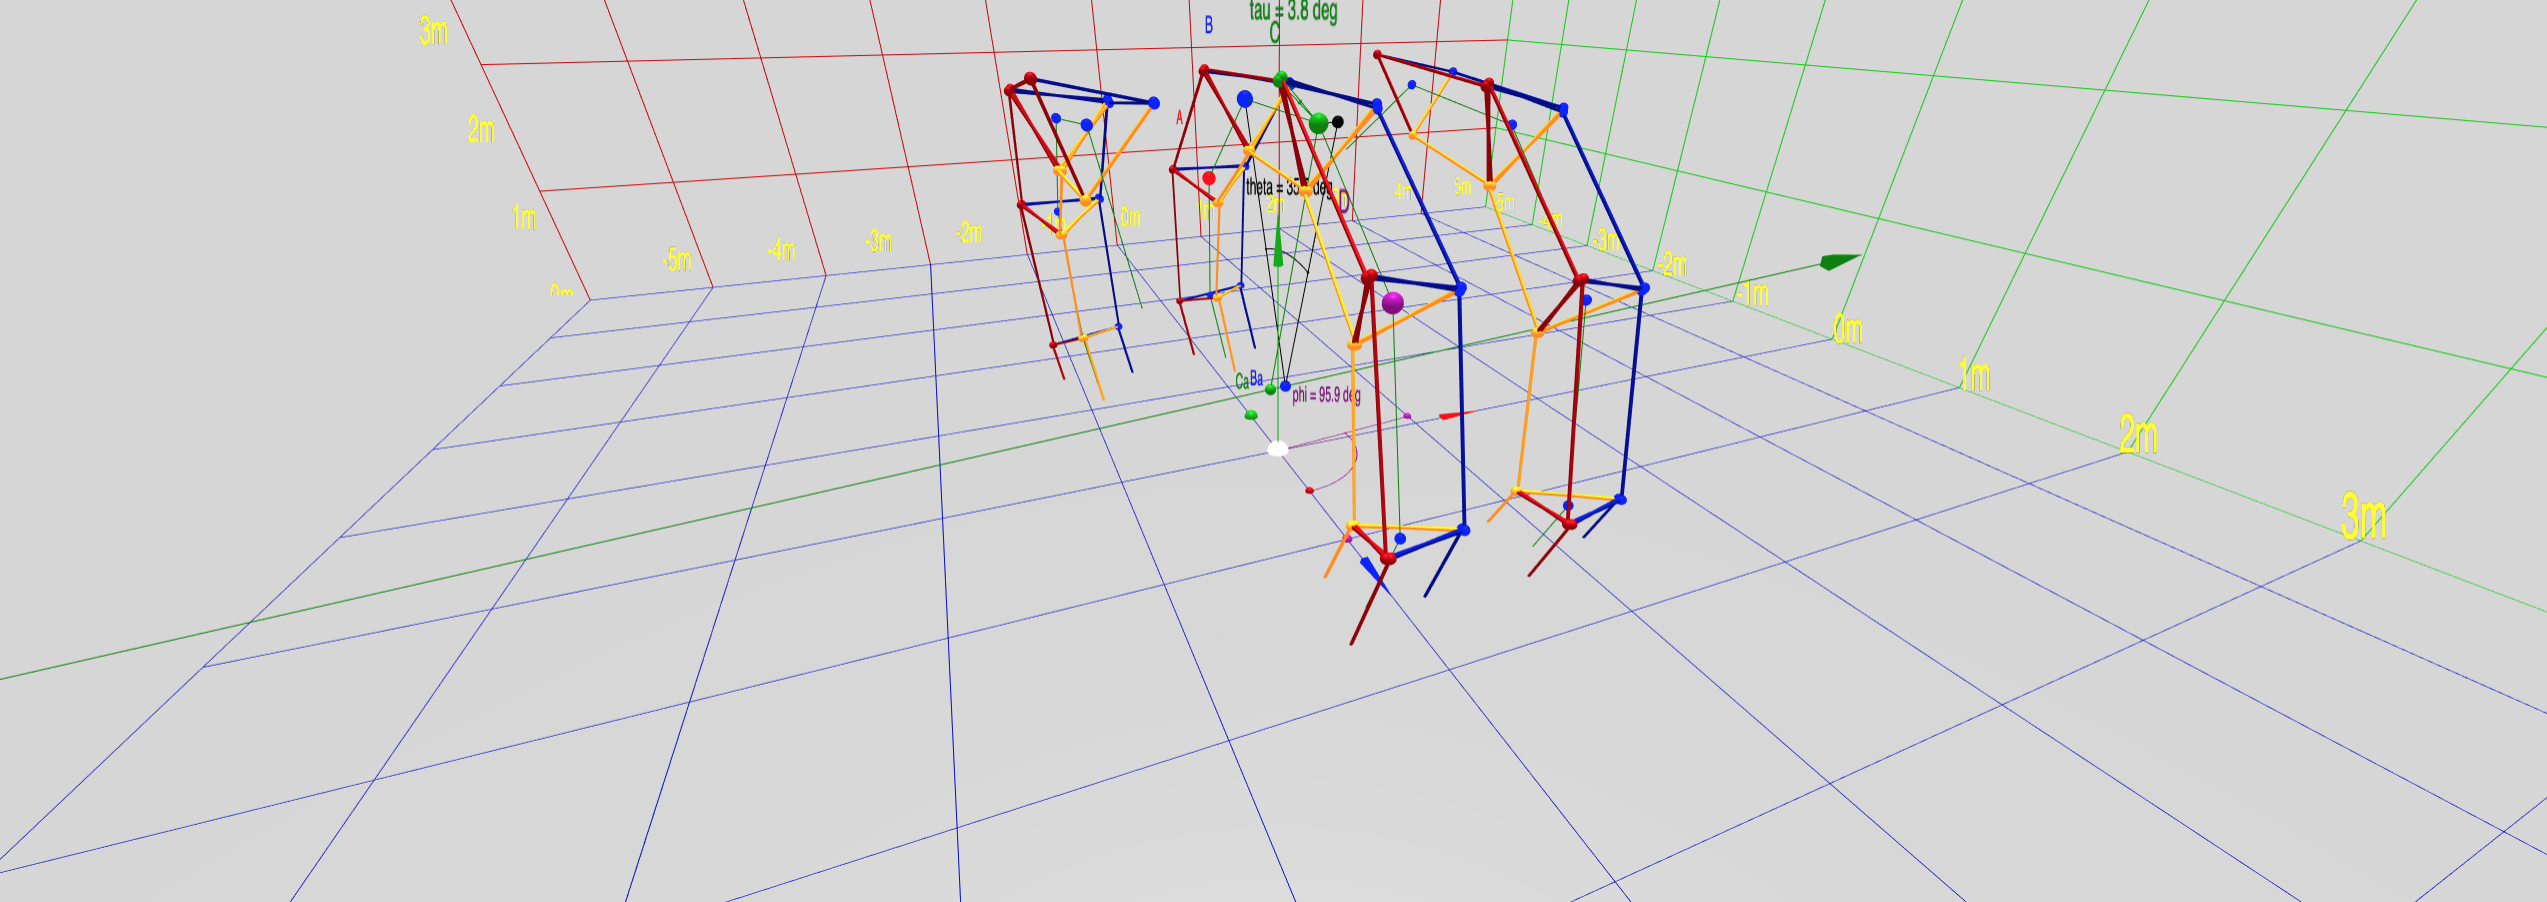
\includegraphics[width=0.32\textwidth]{figures/coiling/tau-375.png}}
%% \caption{$\tau = 0 \degree$}
%% {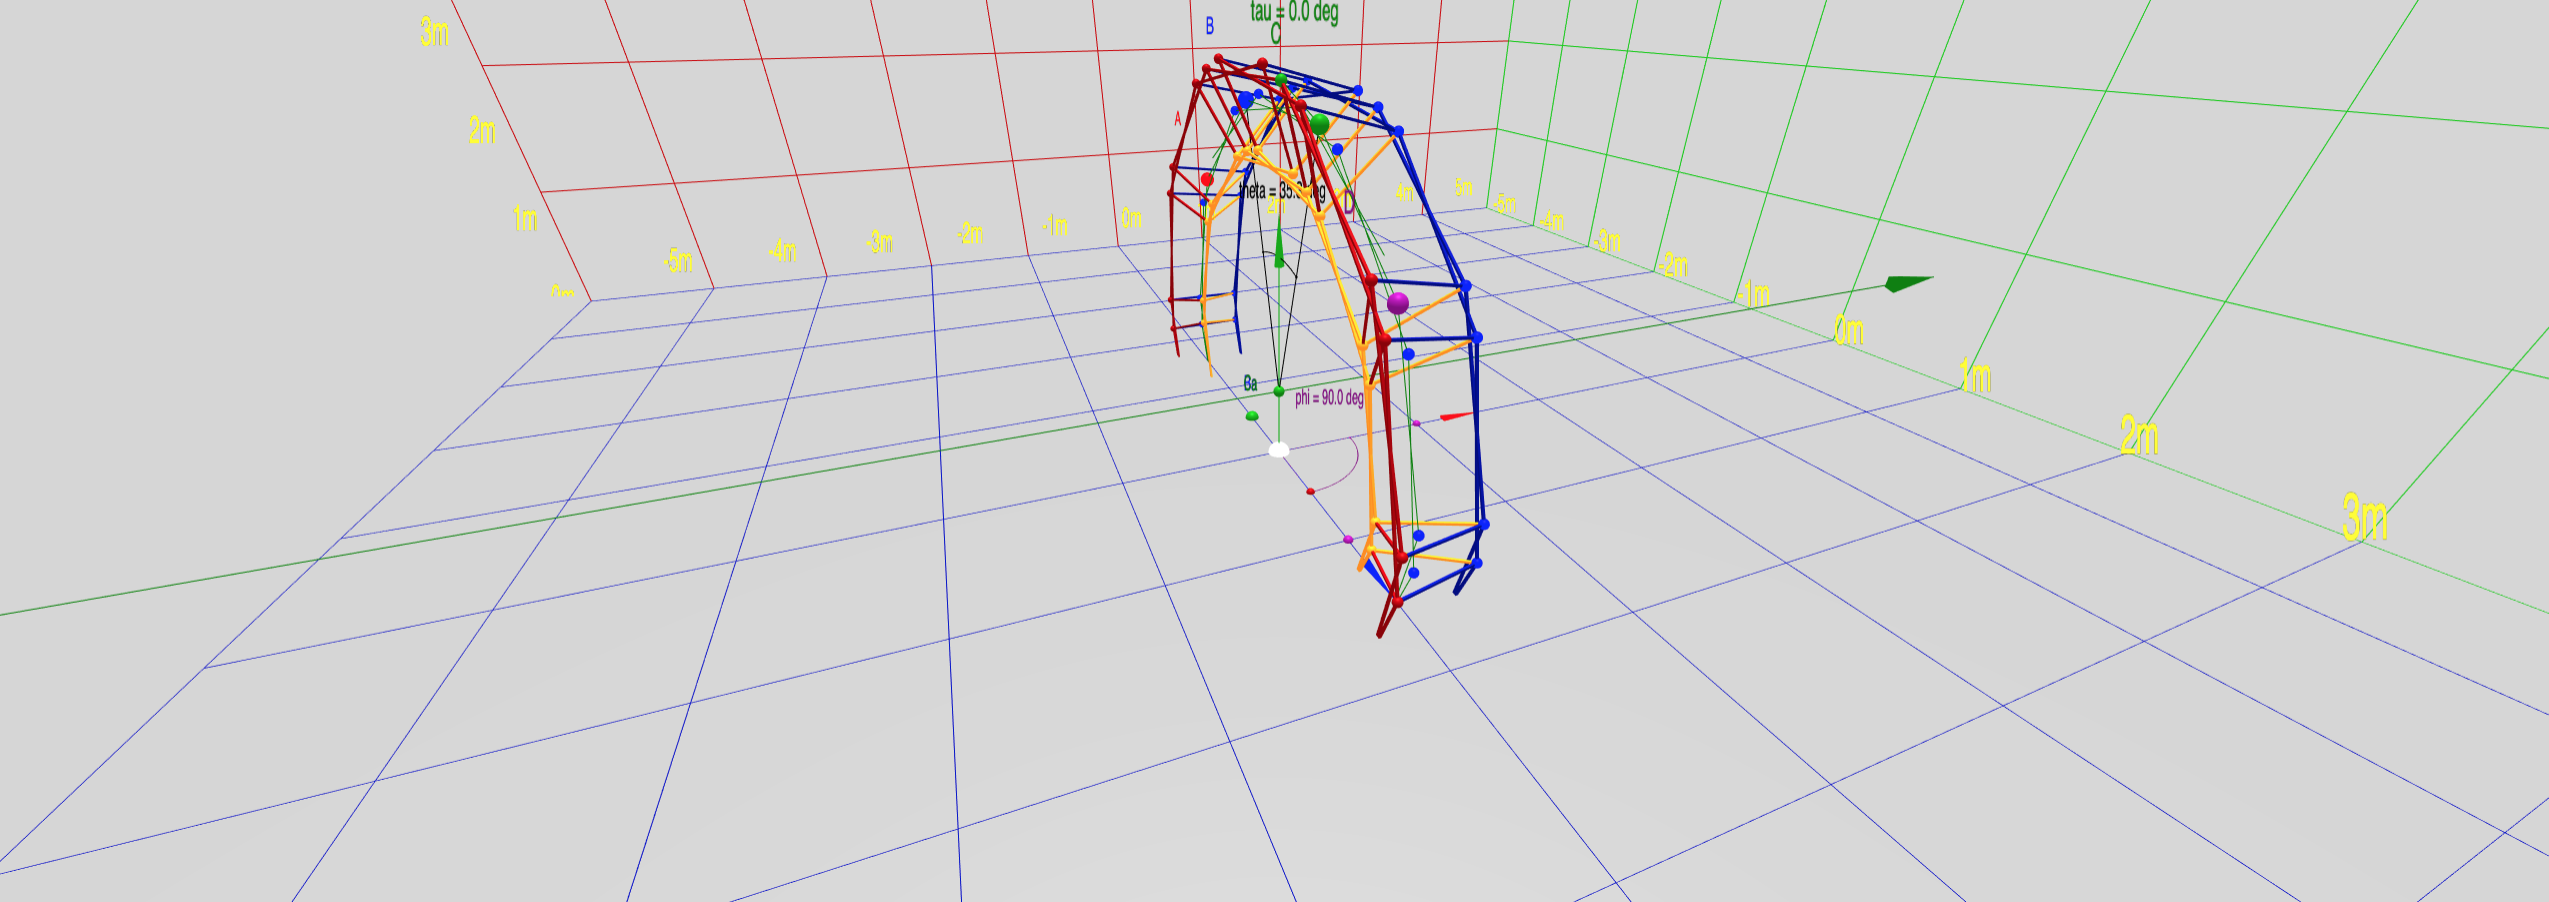
\includegraphics[width=0.32\textwidth]{figures/coiling/tau0.png}}
%% \caption{$\tau = 3.75 \degree$}
%% {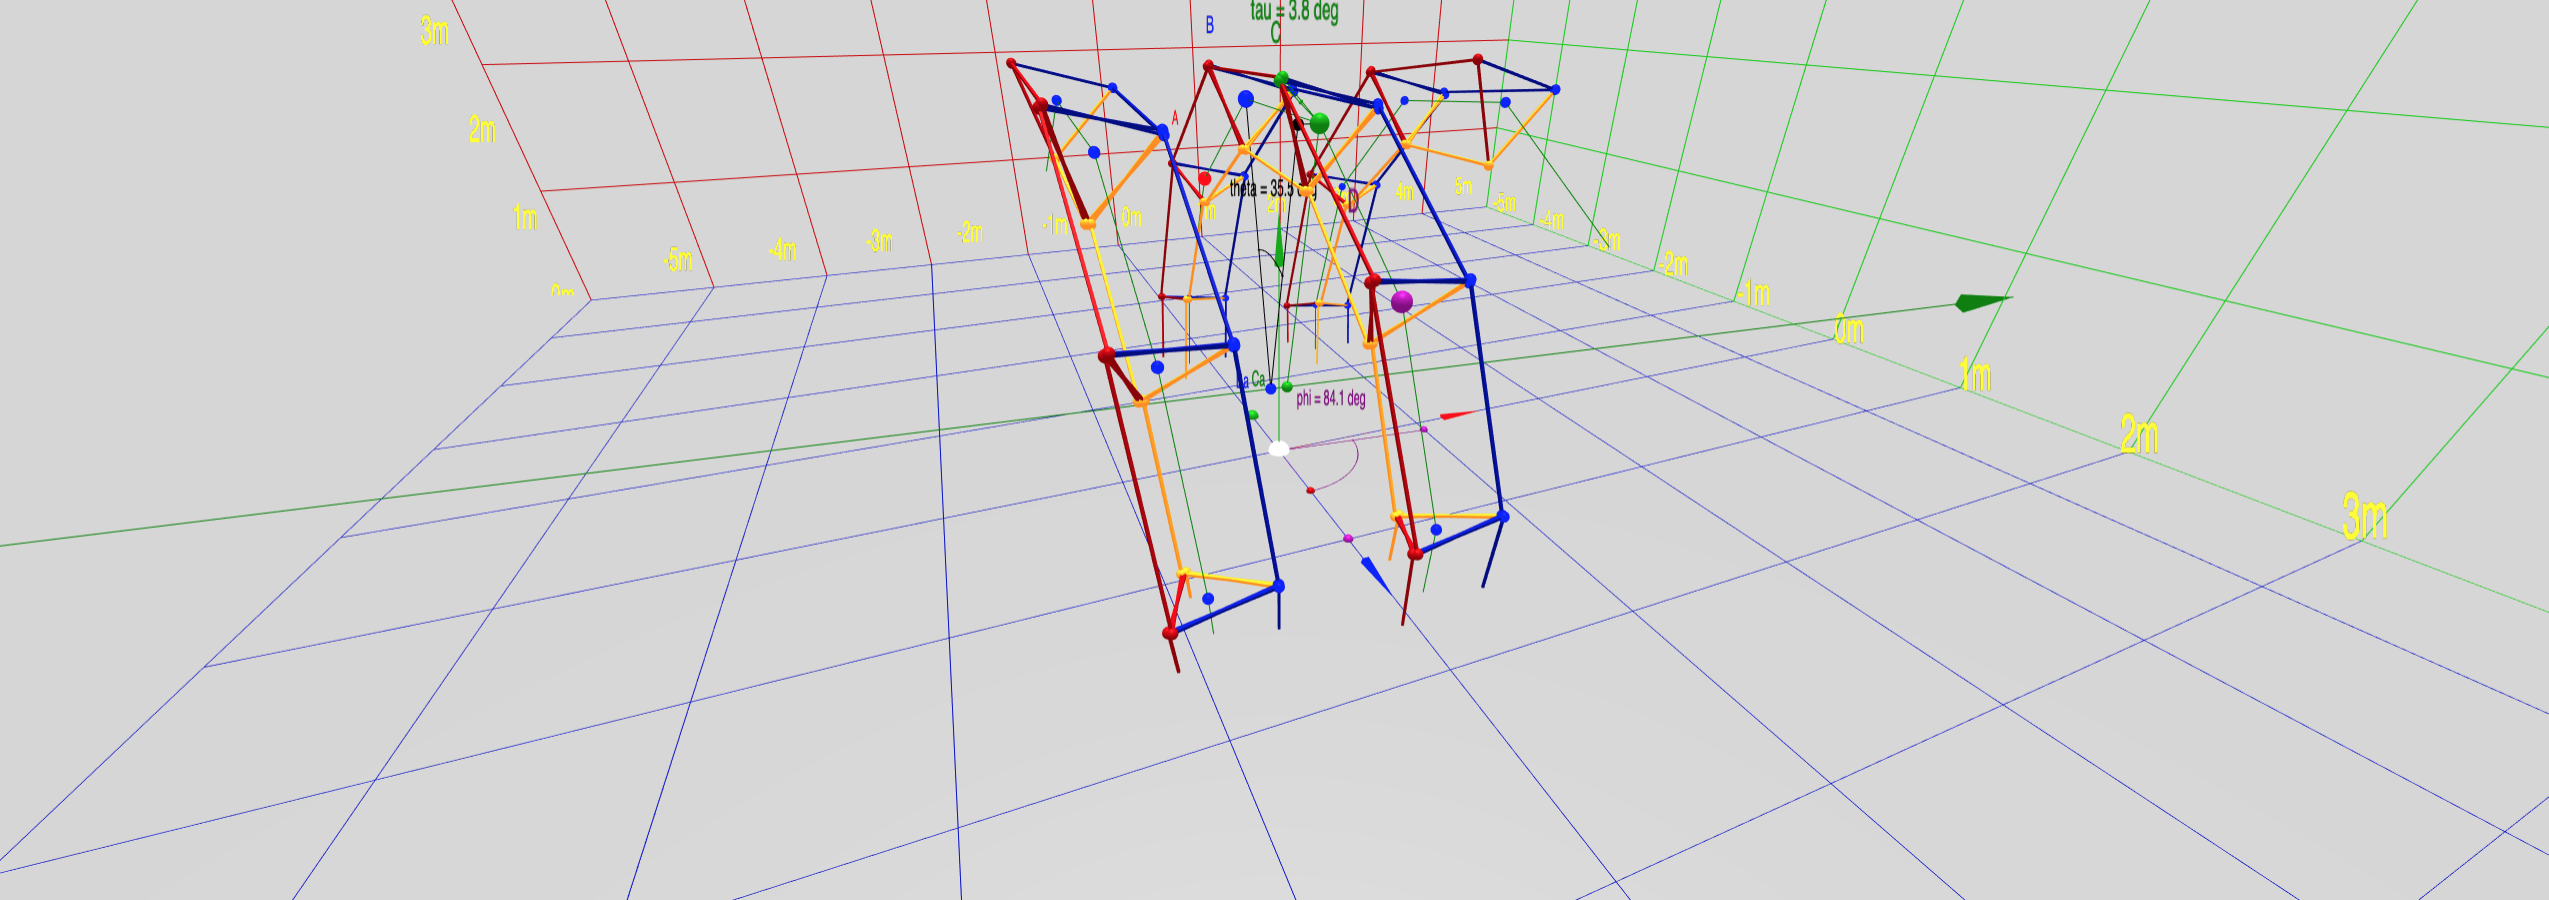
\includegraphics[width=0.32\textwidth]{figures/coiling/tau375.png}}
%%   \caption{$\tau = 7.5 \degree$ }
%% {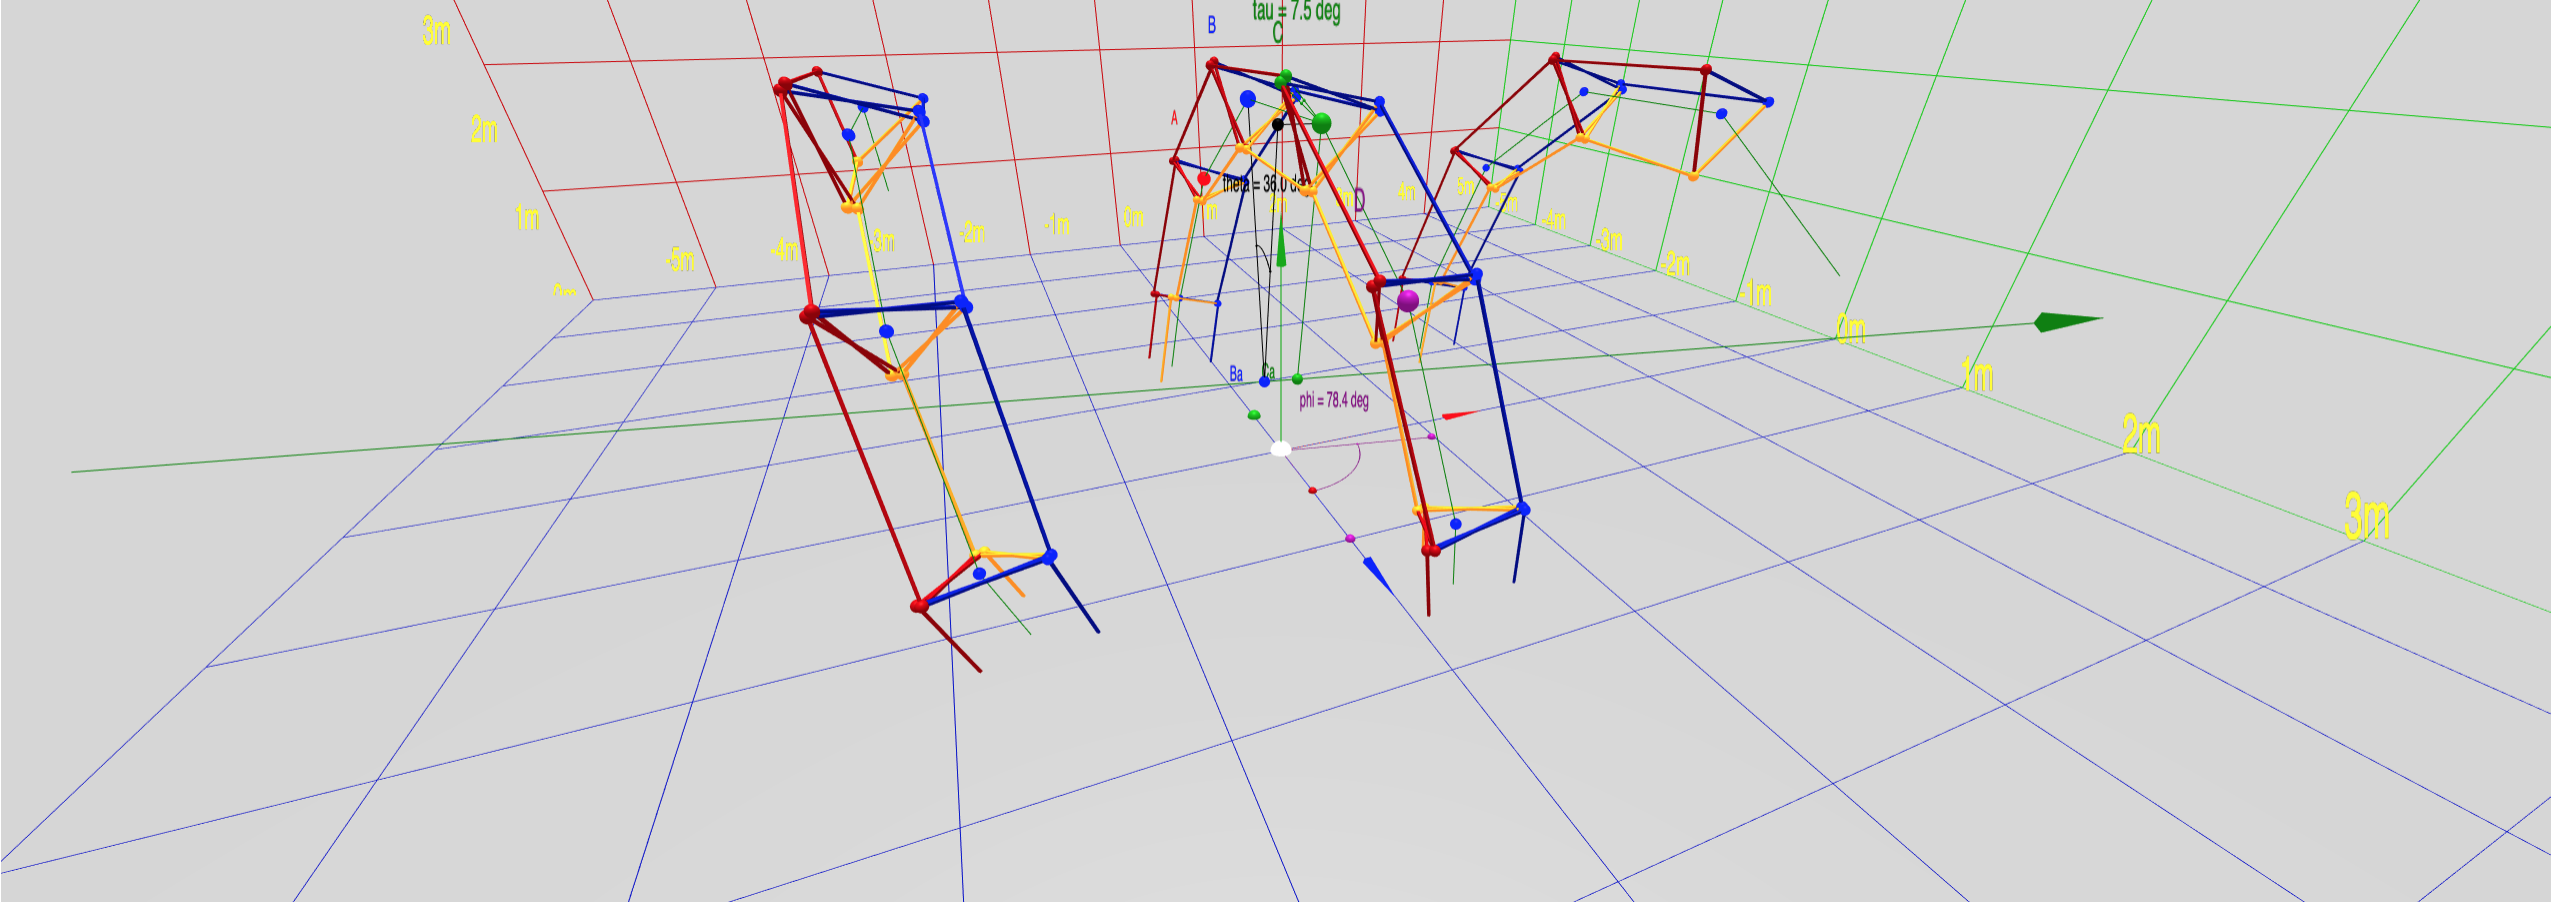
\includegraphics[width=0.32\textwidth]{figures/coiling/tau75.png}}
%%   \caption{$\tau = 15 \degree$ }
%% {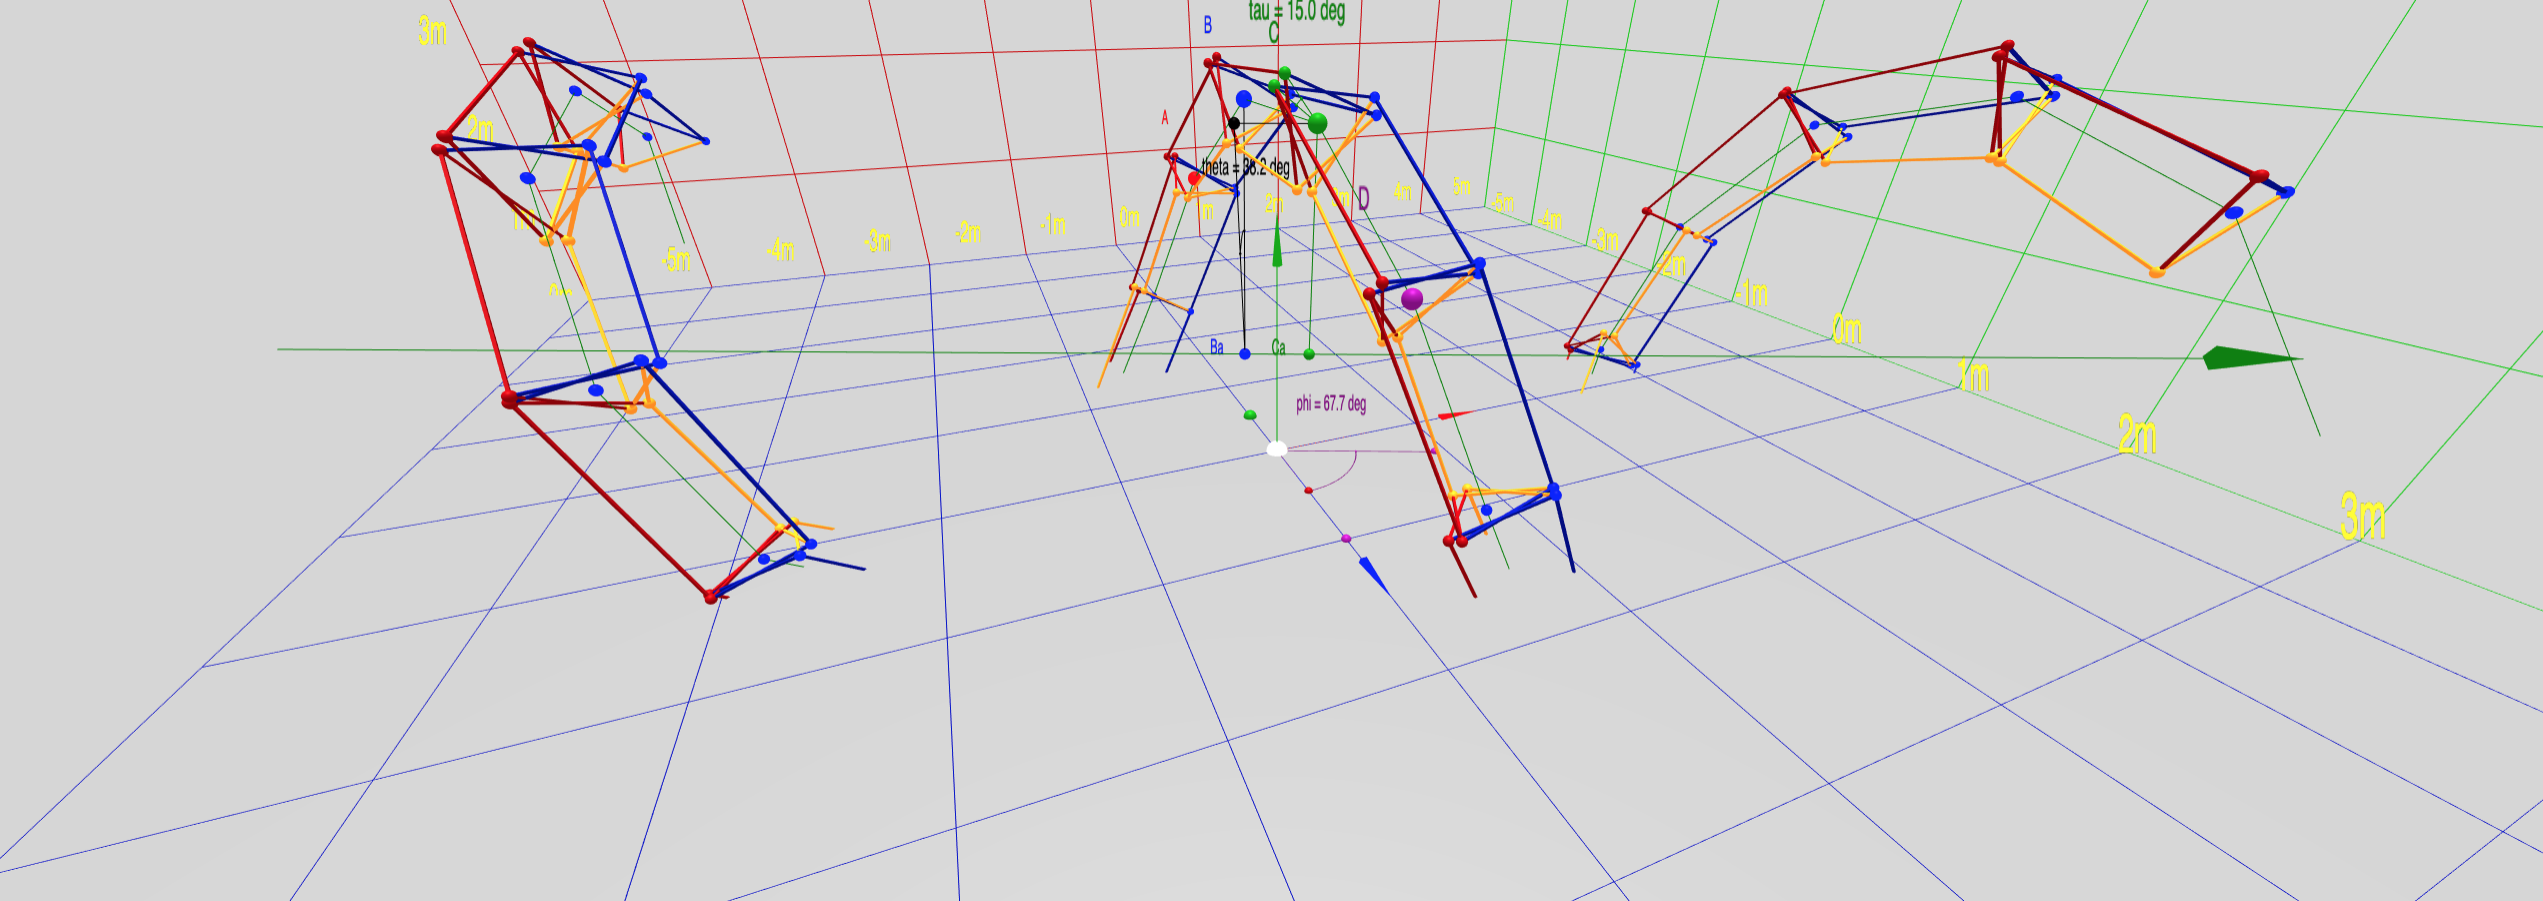
\includegraphics[width=0.32\textwidth]{figures/coiling/tau15.png}}
%% \caption{$\tau = 30 \degree$}
%% {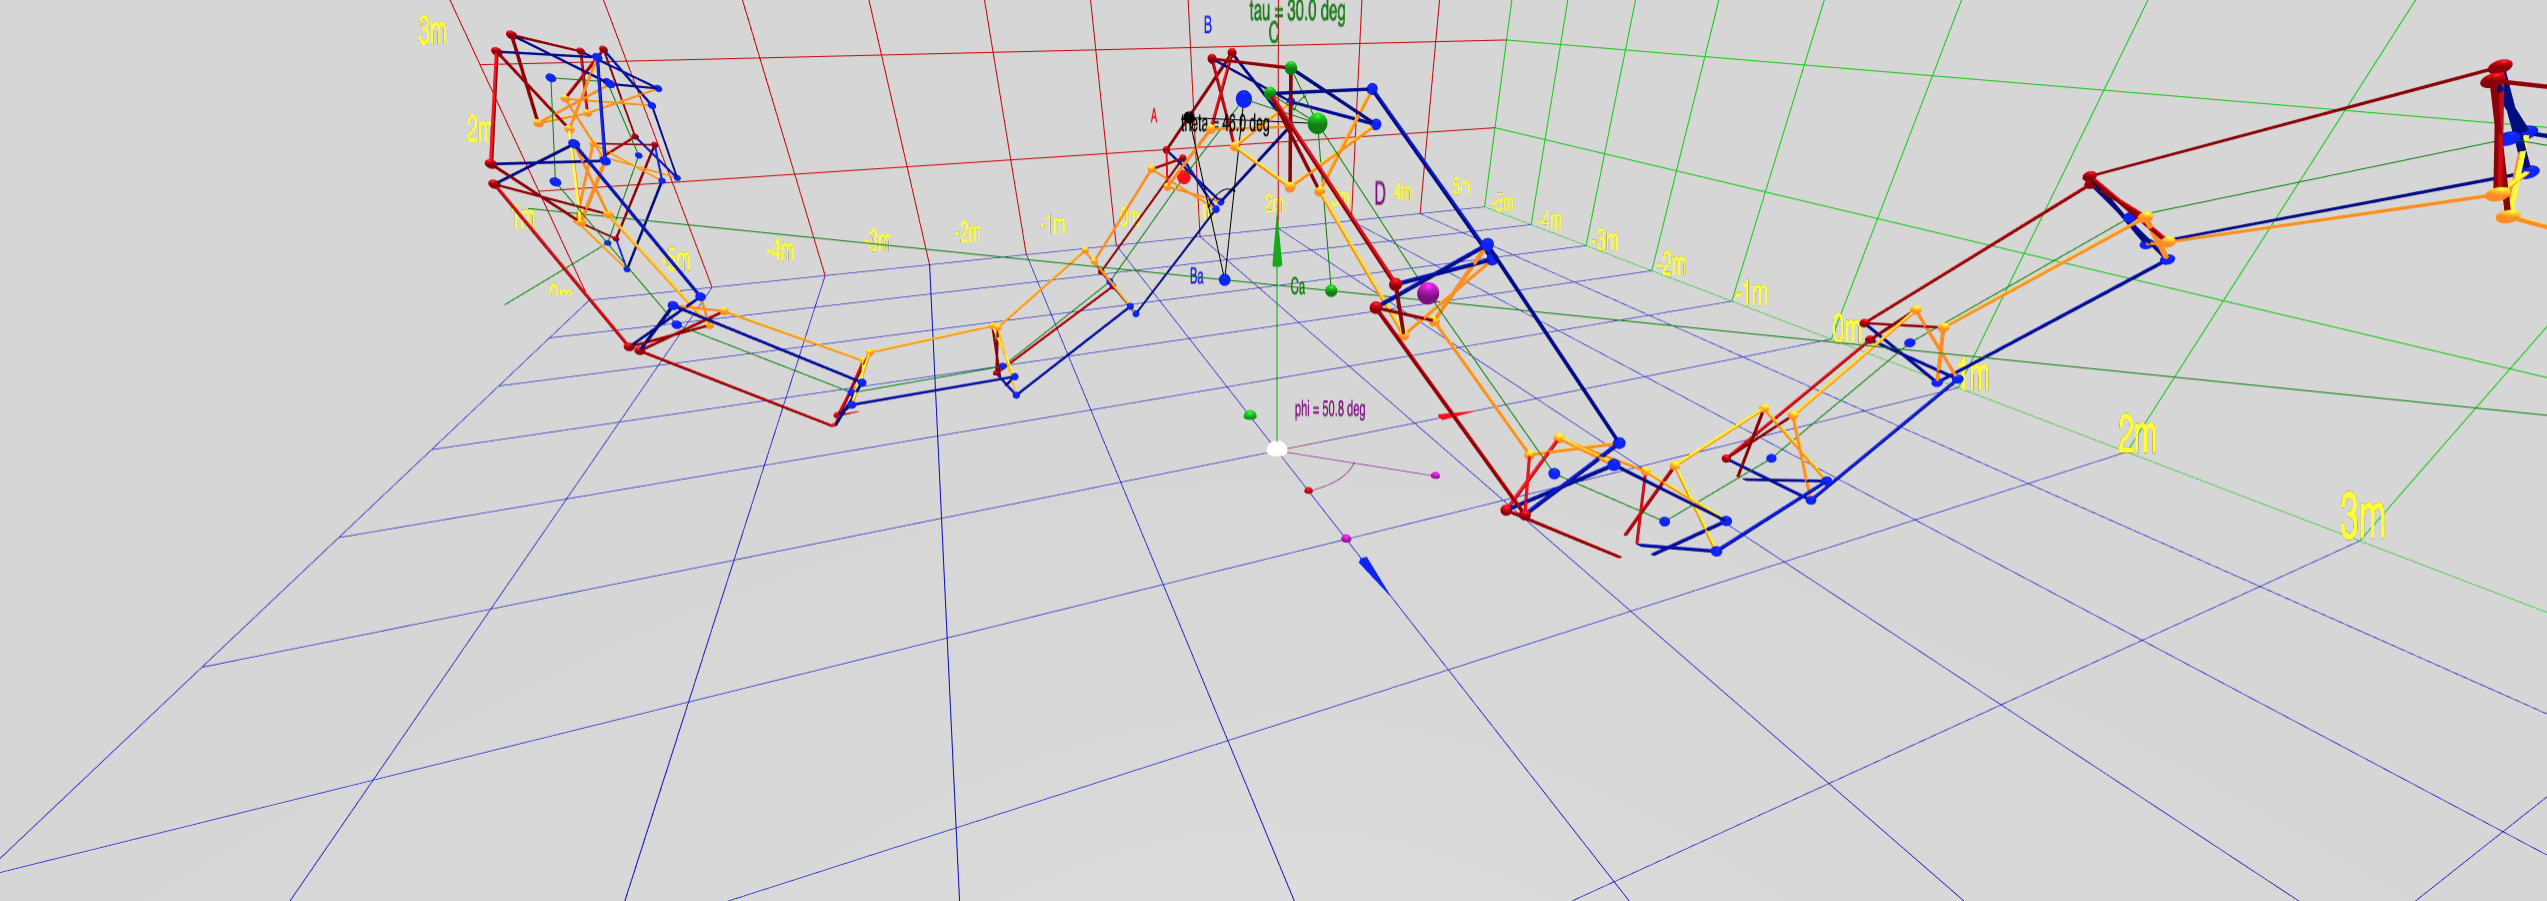
\includegraphics[width=0.32\textwidth]{figures/coiling/tau30.png}}
%% \caption{$\tau = 60 \degree$}
%% {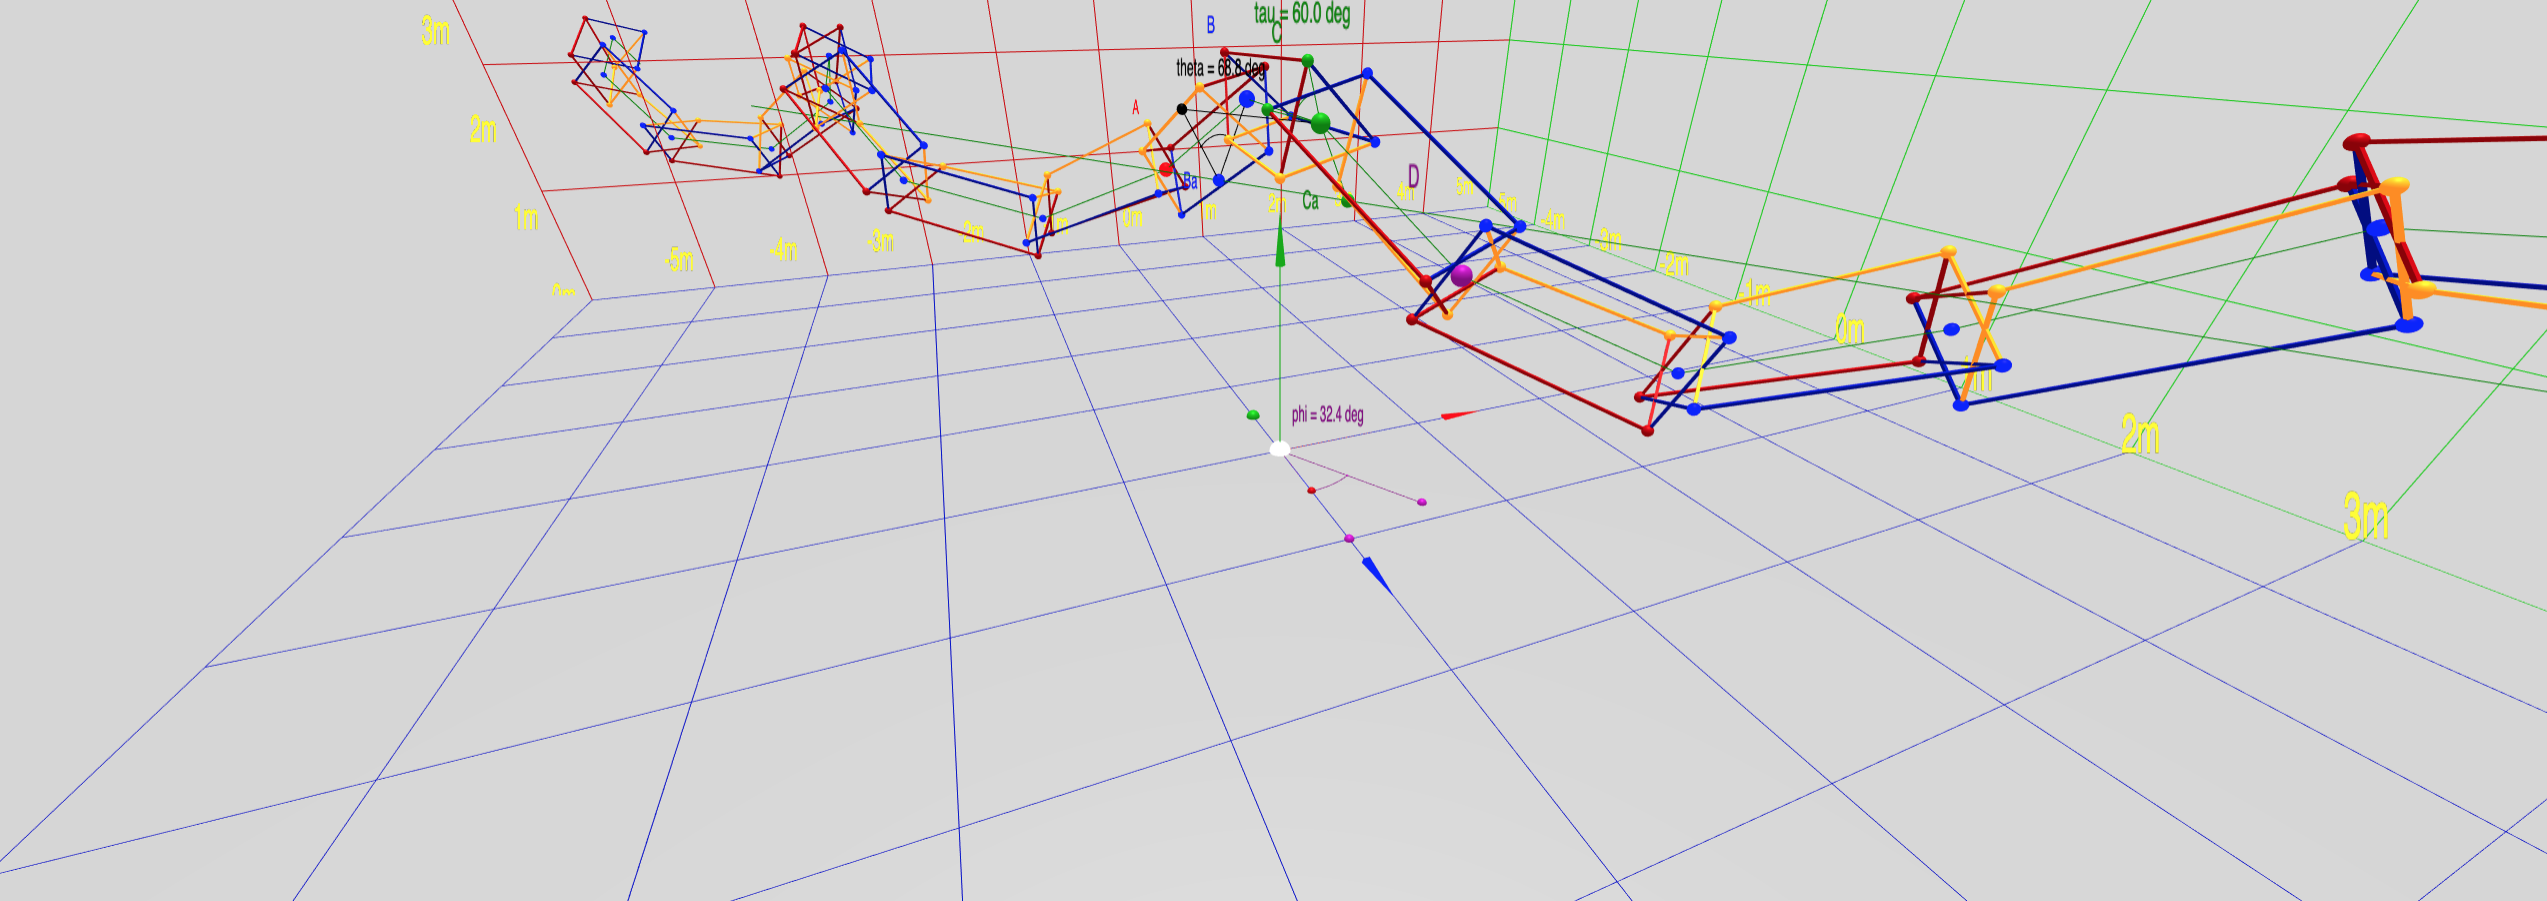
\includegraphics[width=0.32\textwidth]{figures/coiling/tau60.png}}
%% \caption{$\tau = 120 \degree$}
%% {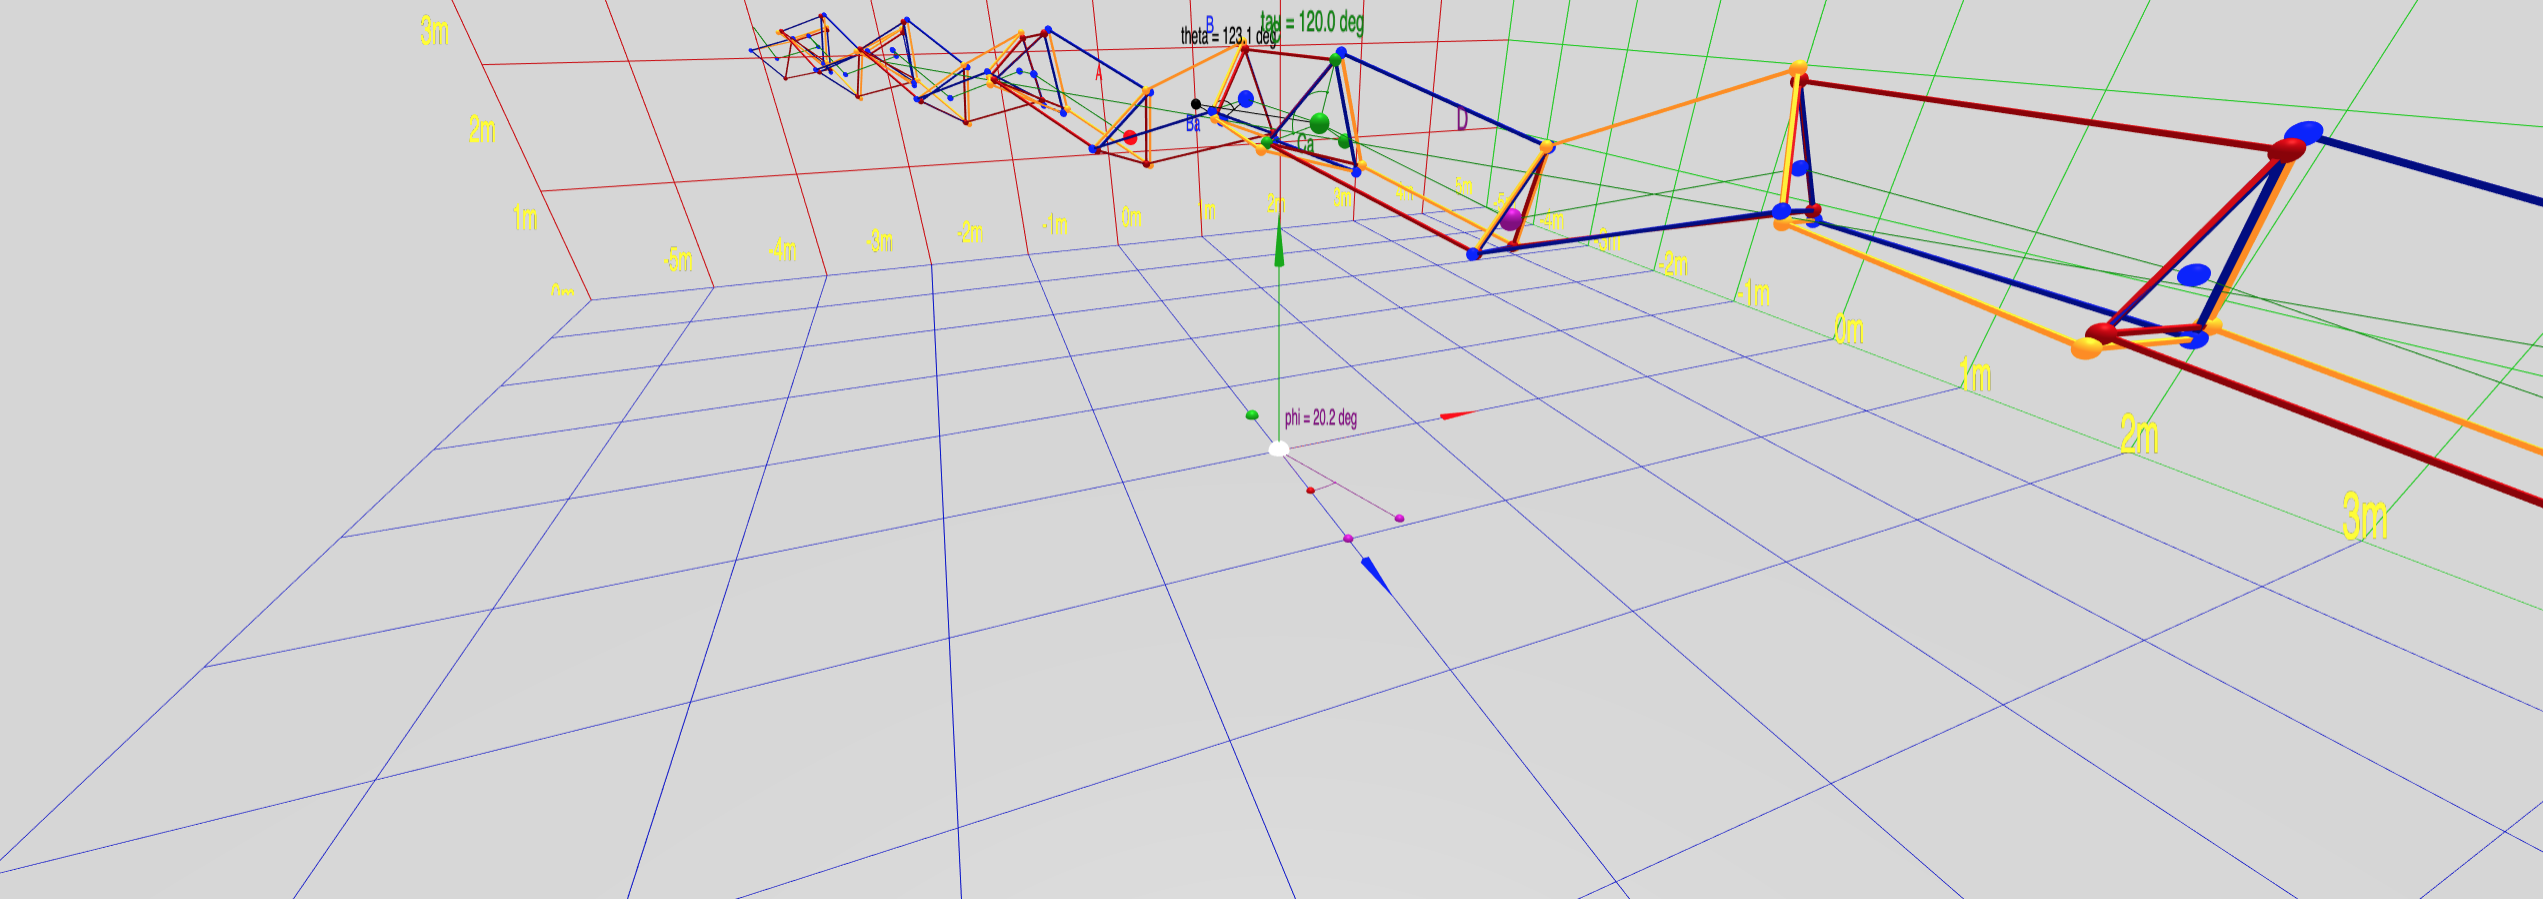
\includegraphics[width=0.32\textwidth]{figures/coiling/tau120.png}}
%% \caption{$\tau = 180 \degree$}
  %% {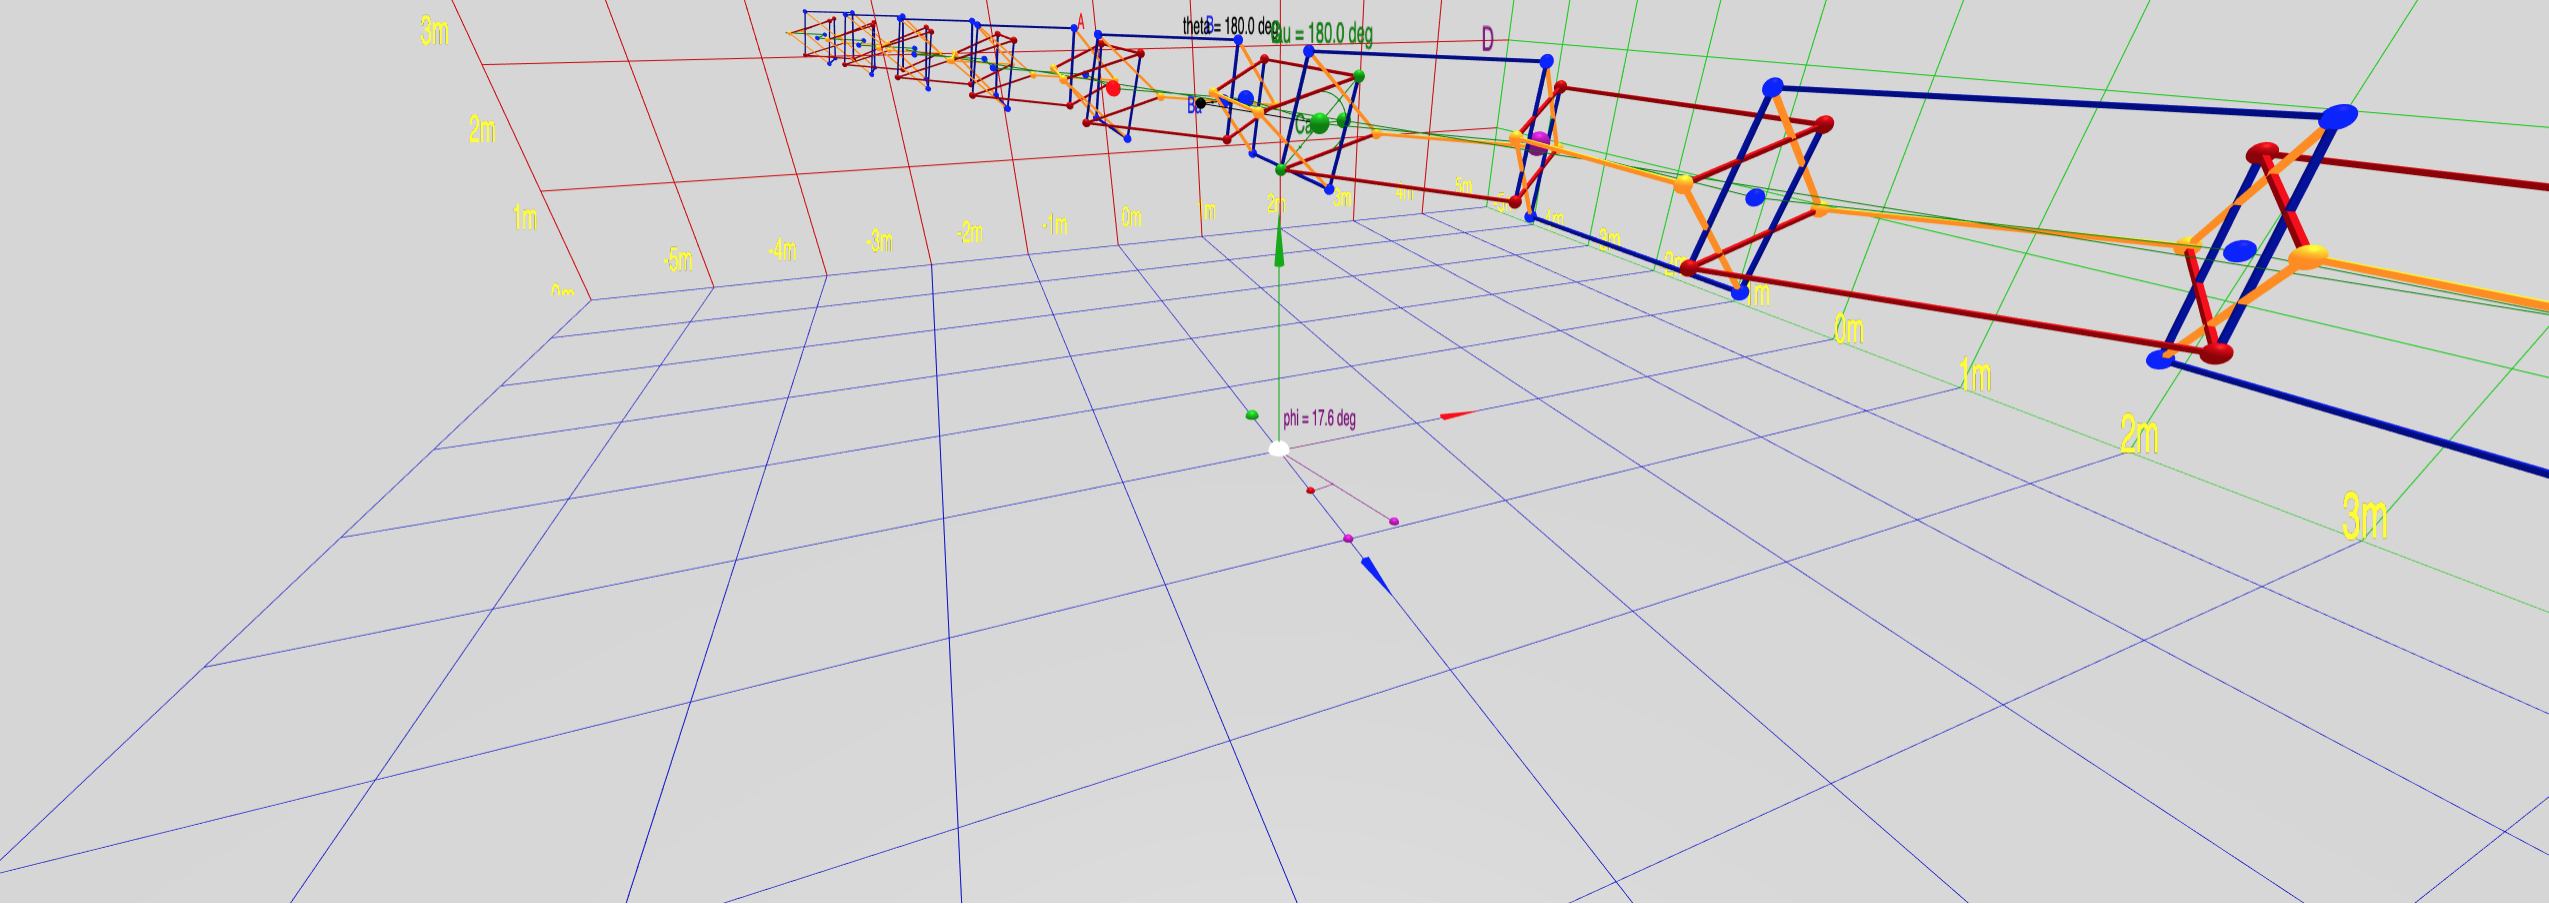
\includegraphics[width=0.32\textwidth]{figures/coiling/tau180.png}}

{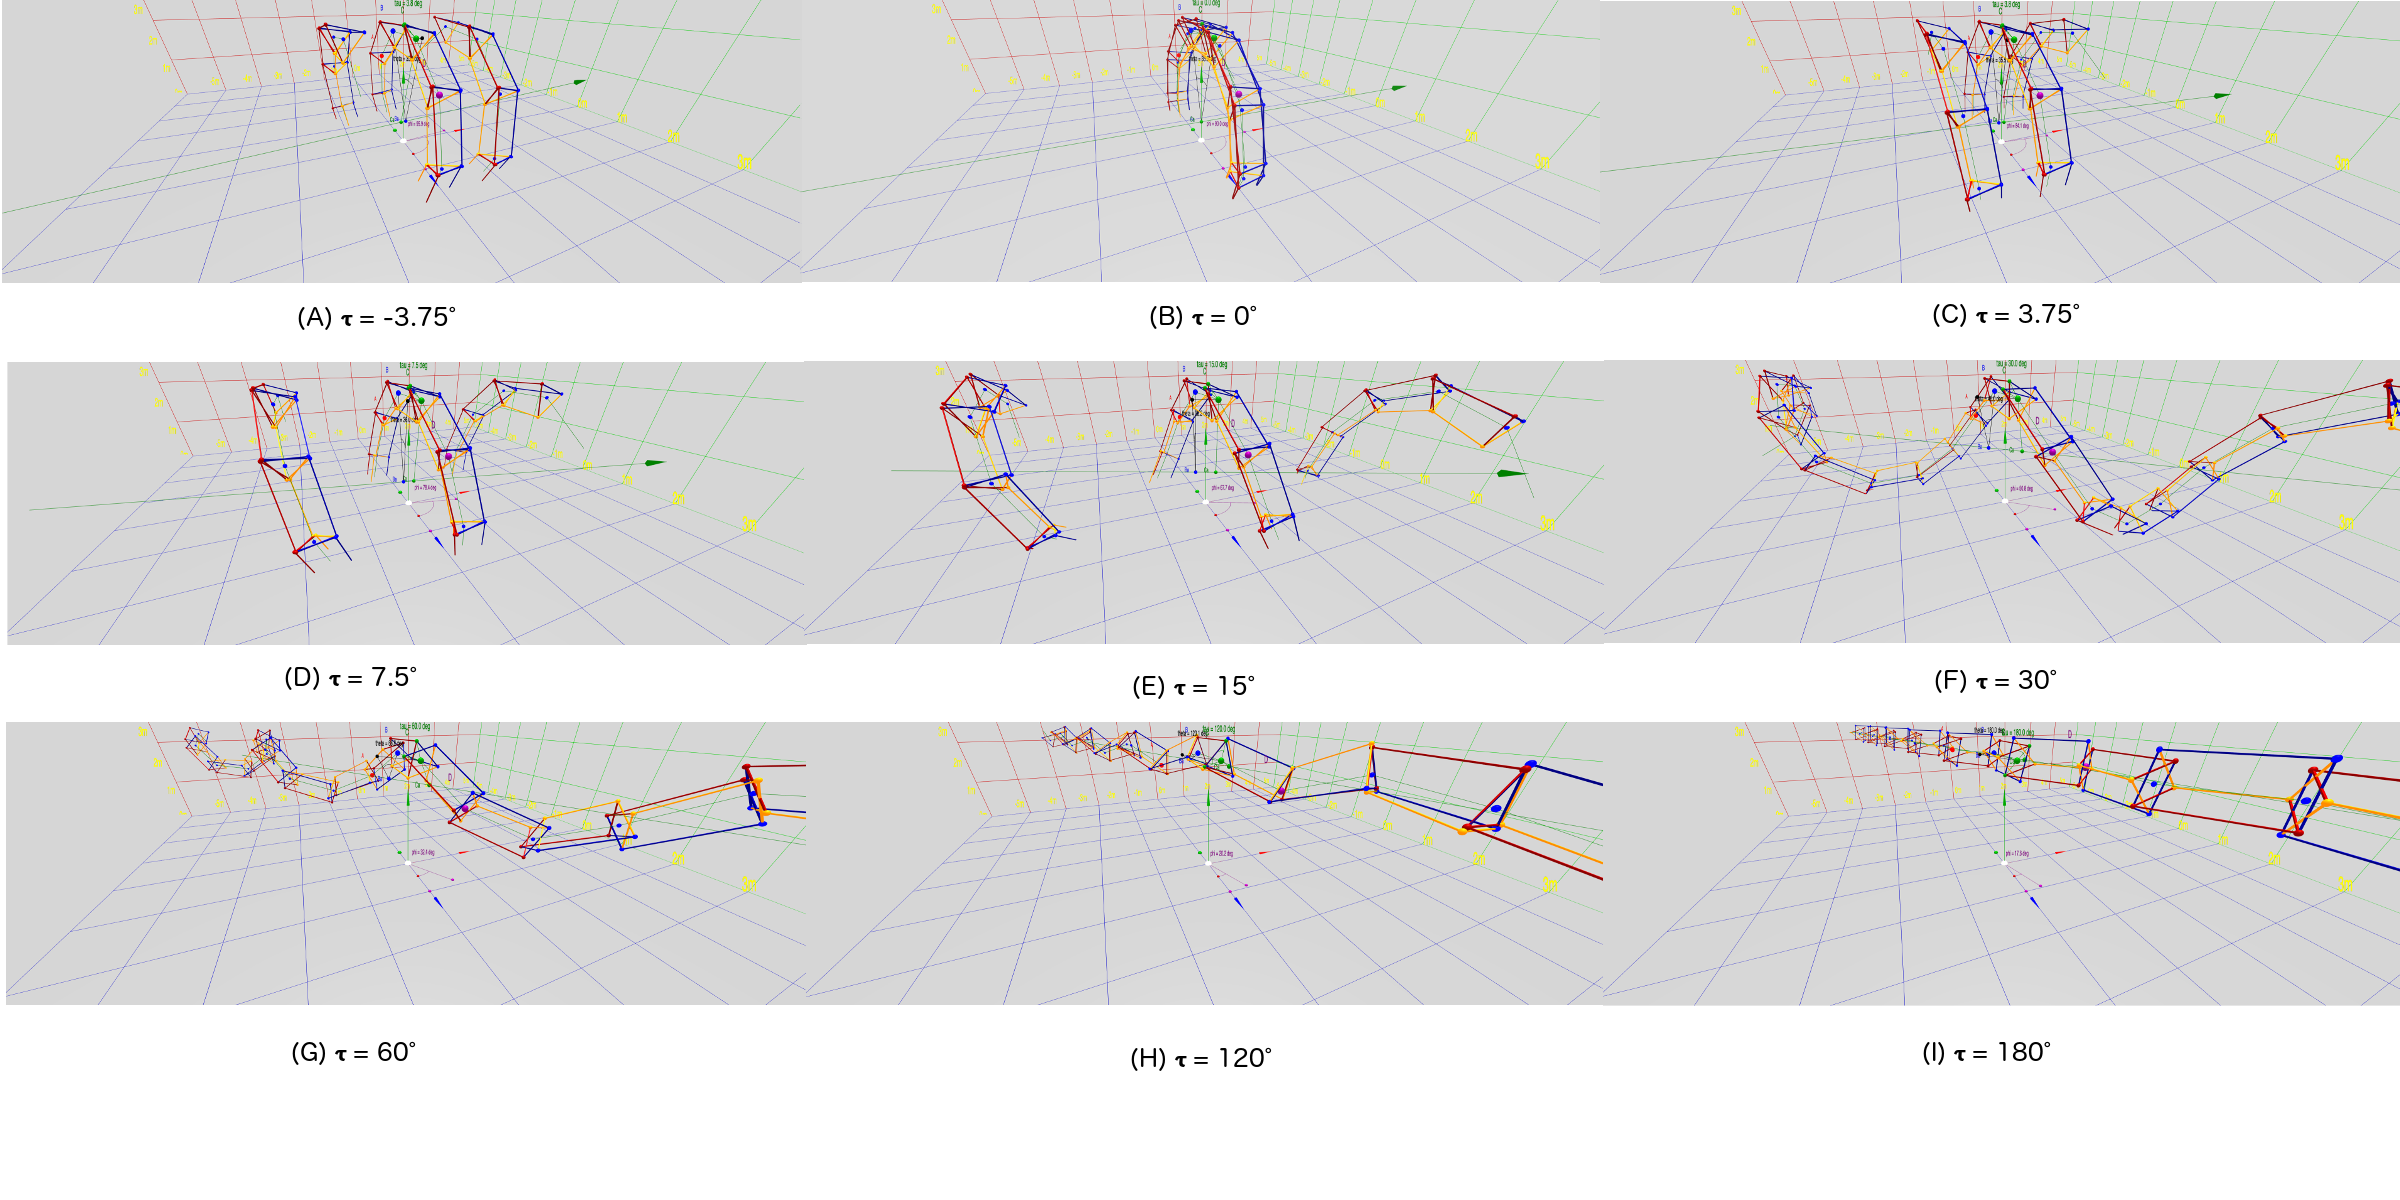
\includegraphics[width=1.0\textwidth]{figures/CoilingFigure.png}}
\caption{Coiling via change to $\tau$}\label{fig:coiling}
\end{figure}

\section{Confirmations and Related Research}

The {\em tetrobot}\cite{TetrobotBook} is the concept of completely
modular robot built entirely out of tetrahedra whose side lengths can
be varied under electronic control. Such robots tend to be inherently
tensegrities\cite{NTRT}, although where the cable lengths
have shrunk to zero.
The current work was instigated by the author's research with a seven-tet tetrobot
displayed in Figure
\ref{fig:tetrobot}.
In particular, it is possible to construct a tentacle, snake-like or
variable-geometry truss configuration of tetrahedra which, in its relaxed
mode, is a regular tetrahelix.

The math in the paper applies to modules of any shape---tetrahedra being
merely an important instance.
The Boerdijk-Coxeter tetrahelix (BC helix) (see Figure \ref{fig:helixnodes}) is a periodic chain of conjoined regular tetrahedra
which has been much studied\cite{coxeter1985simplicial,sadler2019periodic,fuller1982synergetics,read2018transforming}
and happens to have irrational period, making it an ideal
test case for these algorithms/formulae. A recent paper\cite{sadler2019periodic} has explored this
and given an explicit formula for a {\em twist} exactly as defined in this
paper in order to produce a periodic tetrahelix. Both specific instances match the more general results of {\em PointAxis}.

Periodic chains of the five regular Platonic solids joined face-to-face so that their vertices coincide,
which form {\em Platonic helices}\cite{elgersma2016quadrahelix,lord2001sphere}, are completely calculated in a table\cite{readfullsegmentedhelix}.
It is discovered that there are 28 unique members of this ``zoo'' of structures which are occasionally found in chemistry\cite{lord2004gamma,pearce1990structure}.


% \bibliographystyle{unsrt}
\bibliographystyle{plain}
\bibliography{shelix}
\bibstyle{plain}
% \addbibresource{biblio.bib}
% \printbibliography


%% \begin{thebibliography}{6}
%% %

%% \bibitem {smit:wat}
%% Smith, T.F., Waterman, M.S.: Identification of common molecular subsequences.
%% J. Mol. Biol. 147, 195?197 (1981). \url{doi:10.1016/0022-2836(81)90087-5}

%% \bibitem {may:ehr:stein}
%% May, P., Ehrlich, H.-C., Steinke, T.: ZIB structure prediction pipeline:
%% composing a complex biological workflow through web services.
%% In: Nagel, W.E., Walter, W.V., Lehner, W. (eds.) Euro-Par 2006.
%% LNCS, vol. 4128, pp. 1148?1158. Springer, Heidelberg (2006).
%% \url{doi:10.1007/11823285_121}

%% \bibitem {fost:kes}
%% Foster, I., Kesselman, C.: The Grid: Blueprint for a New Computing Infrastructure.
%% Morgan Kaufmann, San Francisco (1999)

%% \bibitem {czaj:fitz}
%% Czajkowski, K., Fitzgerald, S., Foster, I., Kesselman, C.: Grid information services
%% for distributed resource sharing. In: 10th IEEE International Symposium
%% on High Performance Distributed Computing, pp. 181?184. IEEE Press, New York (2001).
%% \url{doi: 10.1109/HPDC.2001.945188}

%% \bibitem {fo:kes:nic:tue}
%% Foster, I., Kesselman, C., Nick, J., Tuecke, S.: The physiology of the grid: an open grid services architecture for distributed systems integration. Technical report, Global Grid
%% Forum (2002)

%% \bibitem {onlyurl}
%% National Center for Biotechnology Information. \url{http://www.ncbi.nlm.nih.gov}



%% \end{thebibliography}
\end{document}


%% \section{Fixed-Period Problems: The Sublinear Case}
%% %
%% With this chapter, the preliminaries are over, and we begin the search
%% for periodic solutions to Hamiltonian systems. All this will be done in
%% the convex case; that is, we shall study the boundary-value problem
%% \begin{eqnarray*}
%%   \dot{x}&=&JH' (t,x)\\
%%   x(0) &=& x(T)
%% \end{eqnarray*}
%% with $H(t,\cdot)$ a convex function of $x$, going to $+\infty$ when
%% $\left\|x\right\| \to \infty$.

%% %
%% \subsection{Autonomous Systems}
%% %
%% In this section, we will consider the case when the Hamiltonian $H(x)$
%% is autonomous. For the sake of simplicity, we shall also assume that it
%% is $C^{1}$.

%% We shall first consider the question of nontriviality, within the
%% general framework of
%% $\left(A_{\infty},B_{\infty}\right)$-subquadratic Hamiltonians. In
%% the second subsection, we shall look into the special case when $H$ is
%% $\left(0,b_{\infty}\right)$-subquadratic,
%% and we shall try to derive additional information.
%% %
%% \subsubsection{The General Case: Nontriviality.}
%% %
%% We assume that $H$ is
%% $\left(A_{\infty},B_{\infty}\right)$-sub\-qua\-dra\-tic at infinity,
%% for some constant symmetric matrices $A_{\infty}$ and $B_{\infty}$,
%% with $B_{\infty}-A_{\infty}$ positive definite. Set:
%% \begin{eqnarray}
%% \gamma :&=&{\rm smallest\ eigenvalue\ of}\ \ B_{\infty} - A_{\infty} \\
%%   \lambda : &=& {\rm largest\ negative\ eigenvalue\ of}\ \
%%   J \frac{d}{dt} +A_{\infty}\ .
%% \end{eqnarray}

%% Theorem~\ref{ghou:pre} tells us that if $\lambda +\gamma < 0$, the
%% boundary-value problem:
%% \begin{equation}
%% \begin{array}{rcl}
%%   \dot{x}&=&JH' (x)\\
%%   x(0)&=&x (T)
%% \end{array}
%% \end{equation}
%% has at least one solution
%% $\overline{x}$, which is found by minimizing the dual
%% action functional:
%% \begin{equation}
%%   \psi (u) = \int_{o}^{T} \left[\frac{1}{2}
%%   \left(\Lambda_{o}^{-1} u,u\right) + N^{\ast} (-u)\right] dt
%% \end{equation}
%% on the range of $\Lambda$, which is a subspace $R (\Lambda)_{L}^{2}$
%% with finite codimension. Here
%% \begin{equation}
%%   N(x) := H(x) - \frac{1}{2} \left(A_{\infty} x,x\right)
%% \end{equation}
%% is a convex function, and
%% \begin{equation}
%%   N(x) \le \frac{1}{2}
%%   \left(\left(B_{\infty} - A_{\infty}\right) x,x\right)
%%   + c\ \ \ \forall x\ .
%% \end{equation}

%% %
%% \begin{proposition}
%% Assume $H'(0)=0$ and $ H(0)=0$. Set:
%% \begin{equation}
%%   \delta := \liminf_{x\to 0} 2 N (x) \left\|x\right\|^{-2}\ .
%%   \label{eq:one}
%% \end{equation}

%% If $\gamma < - \lambda < \delta$,
%% the solution $\overline{u}$ is non-zero:
%% \begin{equation}
%%   \overline{x} (t) \ne 0\ \ \ \forall t\ .
%% \end{equation}
%% \end{proposition}
%% %
%% \begin{proof}
%% Condition (\ref{eq:one}) means that, for every
%% $\delta ' > \delta$, there is some $\varepsilon > 0$ such that
%% \begin{equation}
%%   \left\|x\right\| \le \varepsilon \Rightarrow N (x) \le
%%   \frac{\delta '}{2} \left\|x\right\|^{2}\ .
%% \end{equation}

%% It is an exercise in convex analysis, into which we shall not go, to
%% show that this implies that there is an $\eta > 0$ such that
%% \begin{equation}
%%   f\left\|x\right\| \le \eta
%%   \Rightarrow N^{\ast} (y) \le \frac{1}{2\delta '}
%%   \left\|y\right\|^{2}\ .
%%   \label{eq:two}
%% \end{equation}

%% \begin{figure}
%% \vspace{2.5cm}
%% \caption{This is the caption of the figure displaying a white eagle and
%% a white horse on a snow field}
%% \end{figure}

%% Since $u_{1}$ is a smooth function, we will have
%% $\left\|hu_{1}\right\|_\infty \le \eta$
%% for $h$ small enough, and inequality (\ref{eq:two}) will hold,
%% yielding thereby:
%% \begin{equation}
%%   \psi (hu_{1}) \le \frac{h^{2}}{2}
%%   \frac{1}{\lambda} \left\|u_{1} \right\|_{2}^{2} + \frac{h^{2}}{2}
%%   \frac{1}{\delta '} \left\|u_{1}\right\|^{2}\ .
%% \end{equation}

%% If we choose $\delta '$ close enough to $\delta$, the quantity
%% $\left(\frac{1}{\lambda} + \frac{1}{\delta '}\right)$
%% will be negative, and we end up with
%% \begin{equation}
%%   \psi (hu_{1}) < 0\ \ \ \ \ {\rm for}\ \ h\ne 0\ \ {\rm small}\ .
%% \end{equation}

%% On the other hand, we check directly that $\psi (0) = 0$. This shows
%% that 0 cannot be a minimizer of $\psi$, not even a local one.
%% So $\overline{u} \ne 0$ and
%% $\overline{u} \ne \Lambda_{o}^{-1} (0) = 0$. \qed
%% \end{proof}
%% %
%% \begin{corollary}
%% Assume $H$ is $C^{2}$ and
%% $\left(a_{\infty},b_{\infty}\right)$-subquadratic at infinity. Let
%% $\xi_{1},\allowbreak\dots,\allowbreak\xi_{N}$  be the
%% equilibria, that is, the solutions of $H' (\xi ) = 0$.
%% Denote by $\omega_{k}$
%% the smallest eigenvalue of $H'' \left(\xi_{k}\right)$, and set:
%% \begin{equation}
%%   \omega : = {\rm Min\,} \left\{\omega_{1},\dots,\omega_{k}\right\}\ .
%% \end{equation}
%% If:
%% \begin{equation}
%%   \frac{T}{2\pi} b_{\infty} <
%%   - E \left[- \frac{T}{2\pi}a_{\infty}\right] <
%%   \frac{T}{2\pi}\omega
%%   \label{eq:three}
%% \end{equation}
%% then minimization of $\psi$ yields a non-constant $T$-periodic solution
%% $\overline{x}$.
%% \end{corollary}
%% %

%% We recall once more that by the integer part $E [\alpha ]$ of
%% $\alpha \in \bbbr$, we mean the $a\in \bbbz$
%% such that $a< \alpha \le a+1$. For instance,
%% if we take $a_{\infty} = 0$, Corollary 2 tells
%% us that $\overline{x}$ exists and is
%% non-constant provided that:

%% \begin{equation}
%%   \frac{T}{2\pi} b_{\infty} < 1 < \frac{T}{2\pi}
%% \end{equation}
%% or
%% \begin{equation}
%%   T\in \left(\frac{2\pi}{\omega},\frac{2\pi}{b_{\infty}}\right)\ .
%%   \label{eq:four}
%% \end{equation}

%% %
%% \begin{proof}
%% The spectrum of $\Lambda$ is $\frac{2\pi}{T} \bbbz +a_{\infty}$. The
%% largest negative eigenvalue $\lambda$ is given by
%% $\frac{2\pi}{T}k_{o} +a_{\infty}$,
%% where
%% \begin{equation}
%%   \frac{2\pi}{T}k_{o} + a_{\infty} < 0
%%   \le \frac{2\pi}{T} (k_{o} +1) + a_{\infty}\ .
%% \end{equation}
%% Hence:
%% \begin{equation}
%%   k_{o} = E \left[- \frac{T}{2\pi} a_{\infty}\right] \ .
%% \end{equation}

%% The condition $\gamma < -\lambda < \delta$ now becomes:
%% \begin{equation}
%%   b_{\infty} - a_{\infty} <
%%   - \frac{2\pi}{T} k_{o} -a_{\infty} < \omega -a_{\infty}
%% \end{equation}
%% which is precisely condition (\ref{eq:three}).\qed
%% \end{proof}
%% %

%% \begin{lemma}
%% Assume that $H$ is $C^{2}$ on $\bbbr^{2n} \setminus \{ 0\}$ and
%% that $H'' (x)$ is non-de\-gen\-er\-ate for any $x\ne 0$. Then any local
%% minimizer $\widetilde{x}$ of $\psi$ has minimal period $T$.
%% \end{lemma}
%% %
%% \begin{proof}
%% We know that $\widetilde{x}$, or
%% $\widetilde{x} + \xi$ for some constant $\xi
%% \in \bbbr^{2n}$, is a $T$-periodic solution of the Hamiltonian system:
%% \begin{equation}
%%   \dot{x} = JH' (x)\ .
%% \end{equation}

%% There is no loss of generality in taking $\xi = 0$. So
%% $\psi (x) \ge \psi (\widetilde{x} )$
%% for all $\widetilde{x}$ in some neighbourhood of $x$ in
%% $W^{1,2} \left(\bbbr / T\bbbz ; \bbbr^{2n}\right)$.

%% But this index is precisely the index
%% $i_{T} (\widetilde{x} )$ of the $T$-periodic
%% solution $\widetilde{x}$ over the interval
%% $(0,T)$, as defined in Sect.~2.6. So
%% \begin{equation}
%%   i_{T} (\widetilde{x} ) = 0\ .
%%   \label{eq:five}
%% \end{equation}

%% Now if $\widetilde{x}$ has a lower period, $T/k$ say,
%% we would have, by Corollary 31:
%% \begin{equation}
%%   i_{T} (\widetilde{x} ) =
%%   i_{kT/k}(\widetilde{x} ) \ge
%%   ki_{T/k} (\widetilde{x} ) + k-1 \ge k-1 \ge 1\ .
%% \end{equation}

%% This would contradict (\ref{eq:five}), and thus cannot happen.\qed
%% \end{proof}
%% %
%% \paragraph{Notes and Comments.}
%% The results in this section are a
%% refined version of \cite{smit:wat};
%% the minimality result of Proposition
%% 14 was the first of its kind.

%% To understand the nontriviality conditions, such as the one in formula
%% (\ref{eq:four}), one may think of a one-parameter family
%% $x_{T}$, $T\in \left(2\pi\omega^{-1}, 2\pi b_{\infty}^{-1}\right)$
%% of periodic solutions, $x_{T} (0) = x_{T} (T)$,
%% with $x_{T}$ going away to infinity when $T\to 2\pi \omega^{-1}$,
%% which is the period of the linearized system at 0.

%% \begin{table}
%% \caption{This is the example table taken out of {\it The
%% \TeX{}book,} p.\,246}
%% \begin{center}
%% \begin{tabular}{r@{\quad}rl}
%% \hline
%% \multicolumn{1}{l}{\rule{0pt}{12pt}
%%                    Year}&\multicolumn{2}{l}{World population}\\[2pt]
%% \hline\rule{0pt}{12pt}
%% 8000 B.C.  &     5,000,000& \\
%%   50 A.D.  &   200,000,000& \\
%% 1650 A.D.  &   500,000,000& \\
%% 1945 A.D.  & 2,300,000,000& \\
%% 1980 A.D.  & 4,400,000,000& \\[2pt]
%% \hline
%% \end{tabular}
%% \end{center}
%% \end{table}
%% %
%% \begin{theorem} [Ghoussoub-Preiss]\label{ghou:pre}
%% Assume $H(t,x)$ is
%% $(0,\varepsilon )$-subquadratic at
%% infinity for all $\varepsilon > 0$, and $T$-periodic in $t$
%% \begin{equation}
%%   H (t,\cdot )\ \ \ \ \ {\rm is\ convex}\ \ \forall t
%% \end{equation}
%% \begin{equation}
%%   H (\cdot ,x)\ \ \ \ \ {\rm is}\ \ T{\rm -periodic}\ \ \forall x
%% \end{equation}
%% \begin{equation}
%%   H (t,x)\ge n\left(\left\|x\right\|\right)\ \ \ \ \
%%   {\rm with}\ \ n (s)s^{-1}\to \infty\ \ {\rm as}\ \ s\to \infty
%% \end{equation}
%% \begin{equation}
%%   \forall \varepsilon > 0\ ,\ \ \ \exists c\ :\
%%   H(t,x) \le \frac{\varepsilon}{2}\left\|x\right\|^{2} + c\ .
%% \end{equation}

%% Assume also that $H$ is $C^{2}$, and $H'' (t,x)$ is positive definite
%% everywhere. Then there is a sequence $x_{k}$, $k\in \bbbn$, of
%% $kT$-periodic solutions of the system
%% \begin{equation}
%%   \dot{x} = JH' (t,x)
%% \end{equation}
%% such that, for every $k\in \bbbn$, there is some $p_{o}\in\bbbn$ with:
%% \begin{equation}
%%   p\ge p_{o}\Rightarrow x_{pk} \ne x_{k}\ .
%% \end{equation}
%% \qed
%% \end{theorem}
%% %
%% \begin{example} [{{\rm External forcing}}]
%% Consider the system:
%% \begin{equation}
%%   \dot{x} = JH' (x) + f(t)
%% \end{equation}
%% where the Hamiltonian $H$ is
%% $\left(0,b_{\infty}\right)$-subquadratic, and the
%% forcing term is a distribution on the circle:
%% \begin{equation}
%%   f = \frac{d}{dt} F + f_{o}\ \ \ \ \
%%   {\rm with}\ \ F\in L^{2} \left(\bbbr / T\bbbz; \bbbr^{2n}\right)\ ,
%% \end{equation}
%% where $f_{o} : = T^{-1}\int_{o}^{T} f (t) dt$. For instance,
%% \begin{equation}
%%   f (t) = \sum_{k\in \bbbn} \delta_{k} \xi\ ,
%% \end{equation}
%% where $\delta_{k}$ is the Dirac mass at $t= k$ and
%% $\xi \in \bbbr^{2n}$ is a
%% constant, fits the prescription. This means that the system
%% $\dot{x} = JH' (x)$ is being excited by a
%% series of identical shocks at interval $T$.
%% \end{example}
%% %
%% \begin{definition}
%% Let $A_{\infty} (t)$ and $B_{\infty} (t)$ be symmetric
%% operators in $\bbbr^{2n}$, depending continuously on
%% $t\in [0,T]$, such that
%% $A_{\infty} (t) \le B_{\infty} (t)$ for all $t$.

%% A Borelian function
%% $H: [0,T]\times \bbbr^{2n} \to \bbbr$
%% is called
%% $\left(A_{\infty} ,B_{\infty}\right)$-{\it subquadratic at infinity}
%% if there exists a function $N(t,x)$ such that:
%% \begin{equation}
%%   H (t,x) = \frac{1}{2} \left(A_{\infty} (t) x,x\right) + N(t,x)
%% \end{equation}
%% \begin{equation}
%%   \forall t\ ,\ \ \ N(t,x)\ \ \ \ \
%%   {\rm is\ convex\ with\  respect\  to}\ \ x
%% \end{equation}
%% \begin{equation}
%%   N(t,x) \ge n\left(\left\|x\right\|\right)\ \ \ \ \
%%   {\rm with}\ \ n(s)s^{-1}\to +\infty\ \ {\rm as}\ \ s\to +\infty
%% \end{equation}
%% \begin{equation}
%%   \exists c\in \bbbr\ :\ \ \ H (t,x) \le
%%   \frac{1}{2} \left(B_{\infty} (t) x,x\right) + c\ \ \ \forall x\ .
%% \end{equation}

%% If $A_{\infty} (t) = a_{\infty} I$ and
%% $B_{\infty} (t) = b_{\infty} I$, with
%% $a_{\infty} \le b_{\infty} \in \bbbr$,
%% we shall say that $H$ is
%% $\left(a_{\infty},b_{\infty}\right)$-subquadratic
%% at infinity. As an example, the function
%% $\left\|x\right\|^{\alpha}$, with
%% $1\le \alpha < 2$, is $(0,\varepsilon )$-subquadratic at infinity
%% for every $\varepsilon > 0$. Similarly, the Hamiltonian
%% \begin{equation}
%% H (t,x) = \frac{1}{2} k \left\|k\right\|^{2} +\left\|x\right\|^{\alpha}
%% \end{equation}
%% is $(k,k+\varepsilon )$-subquadratic for every $\varepsilon > 0$.
%% Note that, if $k<0$, it is not convex.
%% \end{definition}
%% %

%% \paragraph{Notes and Comments.}
%% The first results on subharmonics were
%% obtained by Rabinowitz in \cite{fo:kes:nic:tue}, who showed the existence of
%% infinitely many subharmonics both in the subquadratic and superquadratic
%% case, with suitable growth conditions on $H'$. Again the duality
%% approach enabled Clarke and Ekeland in \cite{may:ehr:stein} to treat the
%% same problem in the convex-subquadratic case, with growth conditions on
%% $H$ only.

%% Recently, Michalek and Tarantello (see \cite{fost:kes} and \cite{czaj:fitz})
%% have obtained lower bound on the number of subharmonics of period $kT$,
%% based on symmetry considerations and on pinching estimates, as in
%% Sect.~5.2 of this article.

%% %
%% % ---- Bibliography ----
%% %
